% 本科毕业论文选项
\documentclass[bachelor,winfonts,replaceperiod]{jnuthesis} 
% Font: winfonts, sourcefonts, adobefonts, fandolfonts
% modify colrlinks in ‘junthesis.cls’ at line 172
%\usepackage[math]{blindtext}
%\usepackage[version=4]{mhchem}
%\usepackage{subfigure}
%\graphicspath{{Figure/}}
\titlea{含硒表面活性剂囊泡的构筑}
\titleb{与性质研究}
\author{陈育明}
\studentnum{1050115220}
\supervisor{刘雪锋}
\supervisorpos{教授}
\supervisorb{update:}
\supervisorbpos{}
\major{应用化学}
\department{化学与材料工程}
\institute{江南大学}
% 学士学位获得日期,需设置年、月,默认为编译日期。
\bachelordegreeyear{2019}
\bachelordegreemonth{6}

\begin{document}
    % 制作中文封面
    \maketitle
    % 开始前言部分
    \frontmatter
    % 论文的中文摘要
    \begin{abstract}
        刺激响应型表面活性剂在外界刺激手段的作用下,其界面性质和体相溶液性质能够发生变化,常见的
        刺激手段包括光、温度、磁场、酸碱、氧化还原以及酶等,而开关表面活性剂是一类具有刺激响应性且
        能够可逆地调解界面性质的表面活性剂。含硒表面活性剂是一类新型的氧化还原型开关表面活性剂,
        其氧化还原条件温和,响应迅速。囊泡是一种表面活性剂聚集体,其中自发囊泡是易于制备
        且是热力学稳定的体系。具有氧化还原刺激响应性的囊泡体系在软模板或微反应器、药物装载及靶向释放等领域具有
        应用价值。
        
        本论文中制备了两种含硒表面活性剂3-十二烷基硒-1-丙基硫酸钠 (SDSePS) 和11-丁基硒-1-十一烷基硫酸钠
        (SBSeUS),分别将其与阳离子表面活性剂十二烷基三甲基溴化铵 (DTAB) 进行复配,得到了囊泡体系SDSePS/DTAB
        和SBSePS/DTAB。因硒醚可以被温和地氧化和还原,因此该囊泡体系应具有氧化还原刺激响应性。
        论文研究了阴阳离子表面活性剂囊泡的复配最佳摩尔比,并对所构筑囊泡的稳定性、
         耐盐性进行测试,考察了不同浓度下复配体系内聚集体的自组装情况,对囊泡的氧化还原刺激
         响应性进行着重考察。最后对两种阴阳离子表面活性剂复配体系的各方面性质
         进行了比较,发现两种复配体系在还原态时各方面性质具有一致性,但是SDSePS/DTAB复配囊泡体系其易氧化程度
         明显优于SBSePS/DTAB。
        \keywords{开关表面活性剂;含硒表面活性剂;氧化还原刺激响应性;囊泡}
    \end{abstract}
    
    % 论文的英文摘要
    \begin{englishabstract}
        Stimuli-responsive surfactants can change their interfaces and bulk solution properties under the influence of external stimuli.
        Common stimuli include light, temperature, magnetic field, pH, redox reactions and enzymes, etc. While switchable surfactants
        are one type of surfactants that with stimuli-responsive and can change their interfacial properties reversily. Selenium-containing surfactants are a novel type of redox switchable surfactants, which can be oxided and reduced mildly and response rapidly. 
        Vesicle is  one type of surfactant aggregates,  in which spontaneous vesicles are easy to prepare and thermodynamically stable
        systems. The redox responsive vesicles may have applications in fields such as soft template or microreactor, drug delivery
        and targeted release.
        
        Two selenium-containing surfactants, sodium 3-(dodecylselanyl)propyl sulfate (SDSePS) and sodium 
        11-(butylselanyl)undecyl sulfate (SBSeUS), were prepared in this thesis. Two kinds of vesicle systems, SDSePS/DTAB and
        SBSePS/DTAB, were constructed by compounding selenium-containing anionic surfactants with cationic surfactant N,N,N-trimethyldodecan-1-aminium bromide (DTAB). The vesicles are redox
        stimuli-responsive as a result of the selenide can be oxided and reduced mildly. In the thesis, the optimal molar ratios for the 
        catanionic surfactant vesicles are studied, and the stability and salt tolerance of the constructed vesicles were investigated.
        The self-assembly of aggregates in complex systems at different molar ratios and  redox stimuli responsiveness were researched. 
        Finally, the properties of two kinds of catanionic surfactant compound systems were compared. It was found that majority properties
        of the two complex systems were consistent in reduced state, but the vesicles of SDSePS/DTAB are significantly easy  to be oxided than SBSePS/DTAB.
        % 英文关键词。关键词之间用英文半角逗号隔开,末尾无符号。
        \englishkeywords{switchable surfactant, selenium-containing surfactant, redox stimuli-responsive, vesicle}
    \end{englishabstract}
    
    % 生成论文目次
    \tableofcontents
    
    % 开始正文部分
    \mainmatter
    
    \chapter{绪论}\label{chapter:introduction}
    \section{引言}
    表面活性剂 (surfactant, surface active agent) 是一种能够溶于水且可使水的表(界)面张力显著降低的物质,
    传统上认为表面活性剂在很低浓度下仍可显著降低液体表(界)面张力,现在一般认为只要在较低
    浓度下可以显著改变表面性质的物质即可划归表面活性剂的范畴。
    
    表面活性剂分子一般由两部分构成:一部分为疏水(亲油)的非极性基团,通常为八个碳以上的烃链;另一
    部分为亲水的极性基团,例如羧基、羟基、磺酸基、季铵基等。表面活性剂分子既亲水又亲油,故被称为
    两亲分子,最典型的例子是肥皂,具有增溶、润湿等作用。表面活性剂因其乳化、润湿、增溶等优良作用而
    被广泛用于如原油回收、土壤修复、乳液聚合、药物制备等领域\cite{秦勇2009}。
    
    \section{刺激响应型表面活性剂}
    一般情况下,表面活性剂大多具有性能稳定的特点,但在大多数情况下,它只需在某一阶段起作用,之后反而
    会难以分离;另一方面,表面活性剂一般不参与化学反应,直接排放既是一种浪费,同时给环境带来压力
    \cite{秦勇2009}。因此先后发展了多样触发机制的可分解型表面活性剂 (cleavable surfactants) 和开关型表面
    活性剂 (switchable surfactants)。
    
    \subsection{可分解型表面活性剂}
    为应对传统表面活性剂生物降解速率慢及其引起的环境问题,人们开始关注于可分解表面活性剂,设想通过在
    分子内嵌入易断裂化学键以提高生物降解速率(尽管研究中的高效催化降解并不能完全代表实际中微生物也能够
    高效地降解)\cite{tehrani2007},此类可分解表面活性剂在酸碱、光照、加热、酶催化等条件下能够促发分解\cite{hellberg2000}。
    传统表面活性剂一般相对稳定,早在可分解表面活性剂的概念开始发展之前,季铵酯类表面活性剂早已被用作
    纺织品柔软剂,这便是典型的可分解表面活性剂。此外,十二烷基硫酸钠能够进行自催化降解、脂肪酸聚氧乙烯酯
    这一表面活性剂应当在中性或弱碱性条件下使用、羰基类表面活性剂在酸性条件会分解这些可分解表面活性剂
    的分解条件均被人们加以应用\cite{tehrani2007}。
    
    对于可分解表面活性剂,其催化分解的手段主要包括:酶、酸、碱、UV光照、臭氧以及加热等。可分解表面
    活性剂主要包含对酸不稳定类(缩醛类、缩酮类、原酸酯类及硅氧烷基表面活性剂)、对碱不稳定类(季铵酯、
    甜菜碱酯、单烷基(醚)碳酸酯)以及对UV-光照、热及臭氧不稳定的各类表面活性剂\cite{hellberg2000,tehrani2007,shukla2010,narayanan2008}。    
%        \begin{figure}
%            \centering
%            \begin{subfigure}[b]{\textwidth}
%                \centering
%                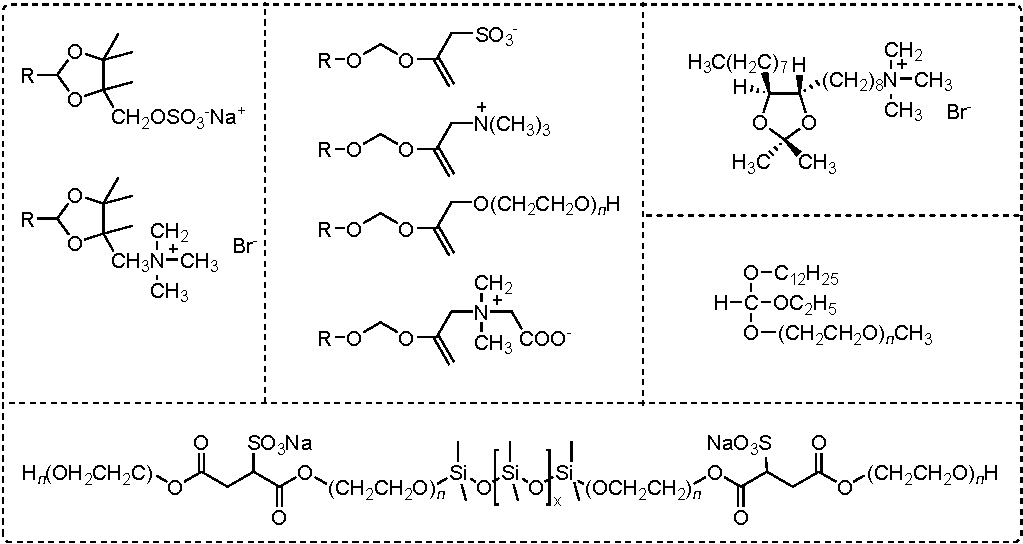
\includegraphics[width=\textwidth]{Figure/cleavable-a.pdf}
%                \caption{对酸性不稳定的可分解表面活性剂}\label{fig:cleavable-a}
%            \end{subfigure}%
%        
%            \begin{subfigure}[b]{\textwidth}
%                \centering
%                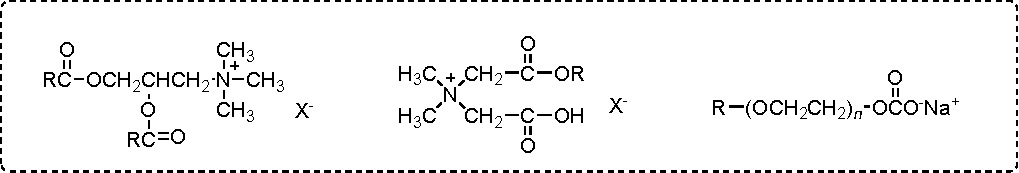
\includegraphics[width=\textwidth]{Figure/cleavable-b.pdf}
%                \caption{对碱性不稳定的可分解表面活性剂}\label{fig:cleavable-b}
%            \end{subfigure}%
%        
%            \begin{subfigure}[b]{\textwidth}
%                \centering
%                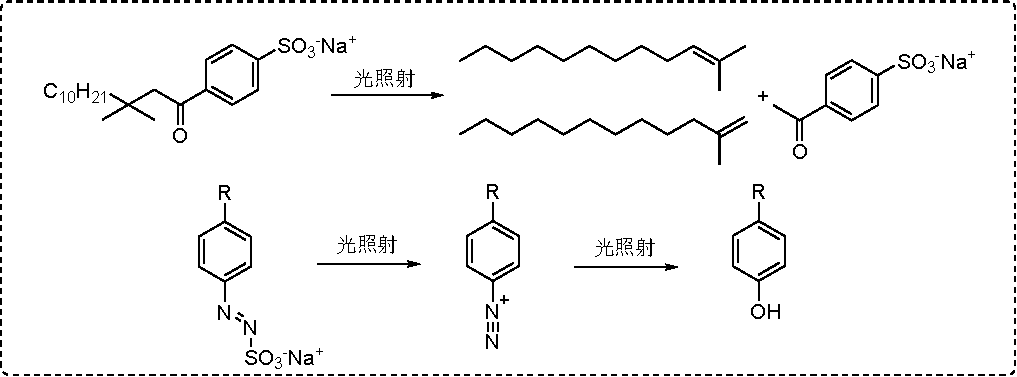
\includegraphics[width=\textwidth]{Figure/cleavable-c.pdf}
%                \caption{光照分解表面活性剂}\label{fig:cleavable-c}
%            \end{subfigure}%
%    
%            \begin{subfigure}[b]{\textwidth}
%                \centering
%                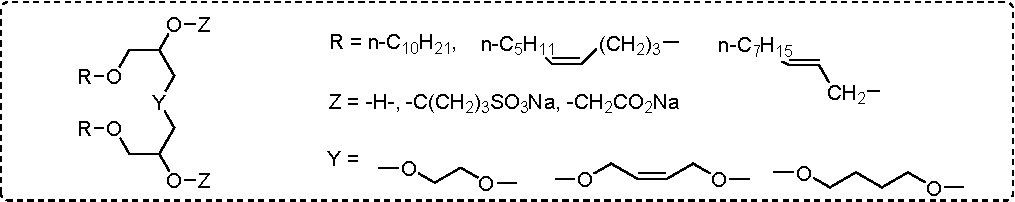
\includegraphics[width=\textwidth]{Figure/cleavable-d.pdf}
%                \caption{臭氧分解表面活性剂}\label{fig:cleavable-d}
%            \end{subfigure}%
%        \end{figure}

%        \begin{figure}[t]
%        \ContinuedFloat
%            \begin{subfigure}[b]{\textwidth}
%                \centering
%                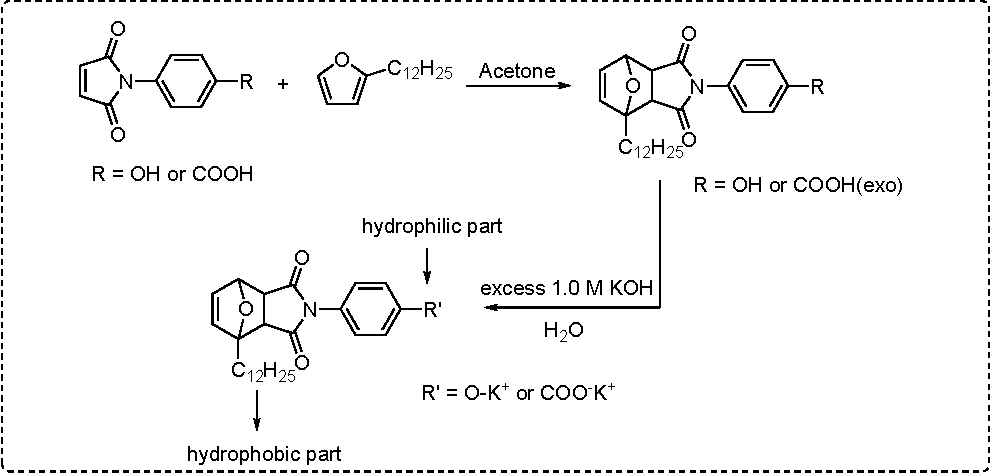
\includegraphics[width=\textwidth]{Figure/cleavable-e.pdf}
%                \caption{臭氧分解表面活性剂}\label{fig:cleavable-e}
%            \end{subfigure}%
%            \caption{已发展的可分解表面活性剂类型}\label{fig:cleavable-saa}
%        \end{figure}
    
    发展可分解表面活性剂最初是面向解决传统表面活性剂难以生物降解带来的环境问题,这一方面已有
    PPS、ProteaseMAX、RapiGest SF等商品化洗涤产品。此外,可分解型表面活性剂亦可用于用于乳液
    破乳、纳米粒子及聚合物制备的模板剂\cite{liu2007}、膜蛋白的质谱分析\cite{norris2003}及胶束电动
    色谱\cite{stanley2012}、囊泡药物装载及释放\cite{guo2012}等方面。但与此同时,化学或酶催化降解
    的可分解表面活性剂或是并不能完全适应于微生物降解\cite{tehrani2007},或是降解速率有待提高,
    更重要的是可分解表面活性剂的分解过程具有不可逆性\cite{liu2007}。
    
%    Liu等\cite{guo2012}以氯化肉豆蔻酰胆碱(及一种季铵酯表面活性剂,在酶催化或碱催化下可分解)及
%    对磺酸杯芳烃(SC4A)构建二级囊泡,利用氯化肉豆蔻酰胆碱在丁酰胆碱酯酶(BChE)作用下酯键
%    断裂,或可应用于阿尔茨海默症的载药及释放(见图\ref{fig:Ch1-SC4A})。
%    \begin{figure}[htbp]
%        \centering
%        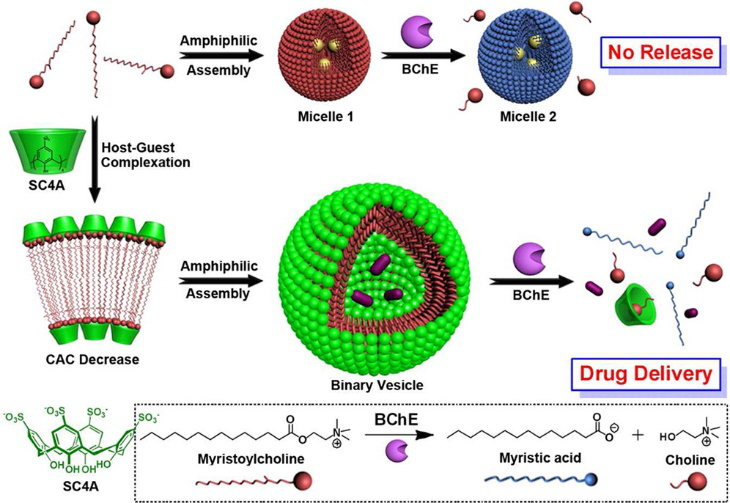
\includegraphics[width= 0.55\textwidth]{Figure/Ch1-SC4A}\\
%        \caption{肉豆蔻酰胆碱在SC4A空白及存在下的两亲自组装示意图}\label{fig:cleavale-SC4A}
%    \end{figure}
    
   \subsection{开关型表面活性剂}
    20世纪80年代以来,开始发展出各种触发机制的开关表面活性剂(switchable surfactants),
    用于可逆地调控表面活性剂性质。例如,需要聚合物乳胶悬浮液在储存运输过程中保持稳定,
    但当其被施工涂刷到物体表面之后,就需要对针对悬浮液“稳定”的性质进行“关闭”,这显然是
    开关表面活性剂的优点\cite{jessop2012},同时这种性质上的“关闭”是可以恢复的,这也是
    相较于可分解型表面活性剂的独到优势。例如,非离子表面活性剂就是一类传统的温度开关
    表面活性剂,当温度上升,其亲水性降低、表面活性降低,但当温度恢复时其性质亦恢复。
    根据这些刺激响应的方式,可以将开关表面活性剂分为:光开关、磁开关、温度开关、酸碱
    开关、\ce{CO2}开关以及氧化还原开关和酶开关表面活性剂\cite{秦勇2009}。
    
    \subsection*{(1) 光开关表面活性剂}
    光开关表面活性剂在非极性疏水尾链或极性亲水头基中具有适当的显色基团\cite{张冤帝2017}。
    根据所需光照条件可将光开关表面活性剂分为两类:一类是稳定型的,利用不同波长的光可
    调节表面活性剂的表面活性;另一类是不稳定的,只有用连续光照才能够实现其表面活性的转变。
    
    根据表面活性剂分子在转变中的变化特点,可以将光开关表面活性剂分为顺反异构型、裂解-聚合型
    以及极性变化型开关表面活性\cite{张冤帝2017,李云霞2011}。顺反异构型开关表面活性剂是
    研究较早的光开关表面活性剂,其主要结构有偶氮苯类、二苯乙烯类以及烷基苯乙烯衍生物等。
    异构型光开关表面活性剂的代表型结构见图\ref{fig:switchable-light}\cite{张冤帝2017,karthaus1996,shang2003,吕湘亮2018}。
    
    \begin{figure}[htbp]
        \centering
        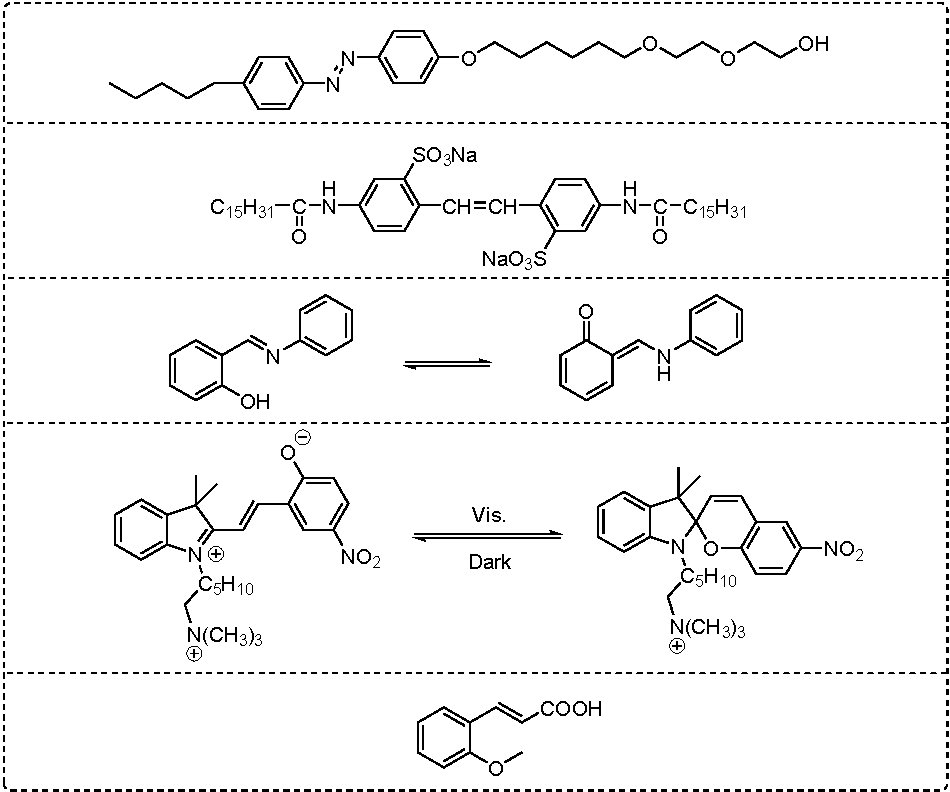
\includegraphics[scale=0.8]{Figure/switchable-light.pdf}\\
        \caption{异构型光开关表面活性剂代表结构\cite{张冤帝2017,karthaus1996,shang2003,吕湘亮2018}}\label{fig:switchable-light}
    \end{figure}
    
    其中,偶氮型光开关表面活性剂研究较早,应用较广,但是一些光敏型表面活性剂\cite{刘清斌2018}如偶氮类分解型及
    光照不可逆型的表面活性剂在使用后并不能可逆地调解、表面活性剂性质不能恢复,应当仅属于刺激响应型表面活性剂
    范畴,不具备开关表面活性剂 (switchable surfaatants) 的属性。
    
    光开关表面活性剂在生物医药、环境修复及减阻传热等方面具有应用价值\cite{刘清斌2018},其中
    关于偶氮类光致异构化的表面活性剂研究较多,Chen等\cite{chen2016}采用偶氮类阳离子表面活性剂
    BTAEAzo实现绿色化的泡沫染整工艺。
    
    除光开关表面活性剂之外,还可以使用具有光刺激响应小分子与表面活性剂作用,构成具有光刺激响应
    的体系。Zhao等\cite{zhao2016}将反式邻甲氧基肉桂酸与N-甲基-N-乙基吡咯烷溴化物(C16MPB)在
    碱性条件下自组装为粘弹性蠕虫状胶束,经UV光照后反式邻甲氧基肉桂酸构型转变,从而使体系转变
    成球形或棒状胶束,见图\ref{fig:switchable-light-omca}。
    
    \begin{figure}[htbp]
        \centering
        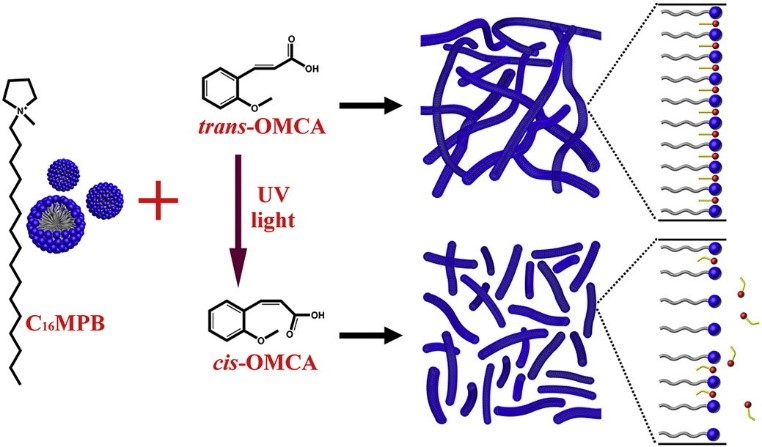
\includegraphics[width=.65\textwidth]{figure/switchable-light-omca.jpg}\\
        \caption{N-甲基-N-乙基吡咯烷溴化物 (C16MPB) 与邻甲氧基肉桂酸构建的光刺激响应性体系\cite{zhao2016}}
        \label{fig:switchable-light-omca}
    \end{figure}
        
    \subsection*{(2) 磁开关表面活性剂}
    磁开关表面活性剂主要为含有磁响应结构,包含离子液体、螯合型以及多金属氧酸盐表面活性剂,
    此外,磁性有机分子表面活性剂是有待发展的新一类磁表面活性剂\cite{brown2015},磁响应表面
    活性剂可用于蛋白质分离、水处理以及环境修复\cite{brown2015}等方面。主要类别磁响应表面活
    性剂见图\ref{fig:switchable-mag}。
    \begin{figure}[htbp]
        \centering
        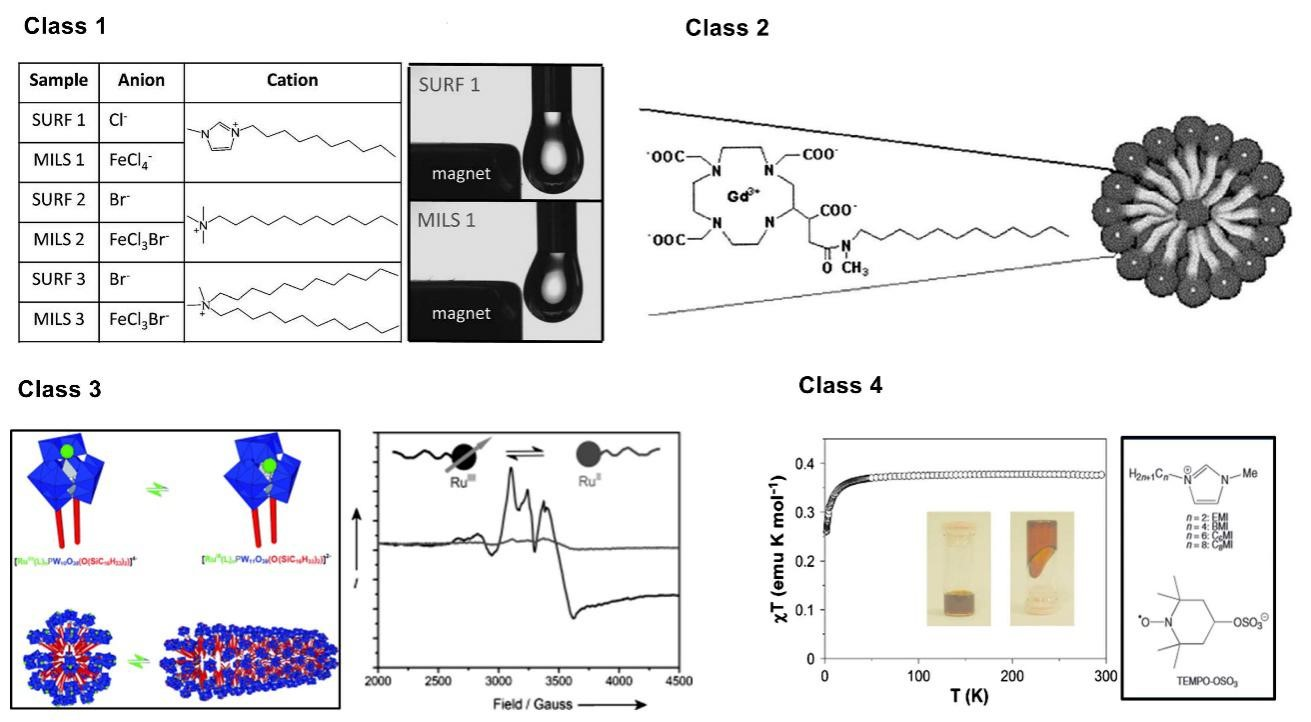
\includegraphics[width=.875\textwidth]{figure/switchable-mag.jpg}\\
        \caption{主要类别的磁开关表面活性剂\cite{brown2015,brown2012}}
        \label{fig:switchable-mag}
    \end{figure}
    
    \subsection*{(3) 温度开关表面活性剂}
    非离子型表面活性剂是典型的温度开关表面活性剂,随温度升高其亲水性会逐渐下降,至浊点时其
    亲水性显著降低,表面活性变差,而当温度降低后其又可恢复表面活性。Chu\cite{chu2011}等以
    棕榈酰氨基磺基甜菜碱 (PDAS) 为表面活性剂制备了一种具有温度响应的凝胶,在 30 ℃ 时形成
    球状或短棒状胶束,在 40 ℃ 时则形成网络蠕虫状胶束%\ref{fig:switchable-temperature}
    ,这是由于加热时疏水部分溶解度降低,
    从而形成网状交联凝胶。
%    \begin{figure}[htbp]
%        \centering
%        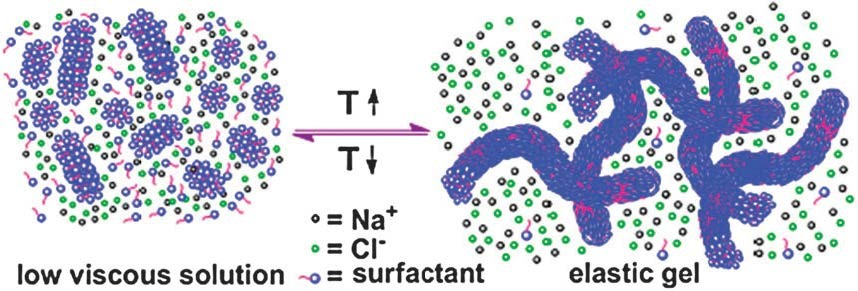
\includegraphics[width=.6\textwidth]{figure/switchable-temperature.jpg}\\
%        \caption{应用温度开关表面活性剂的可转换温感凝胶\cite{chu2011}}
%        \label{fig:switchable-temperature}
%    \end{figure}

    \subsection*{(4) 酸碱开关表面活性剂}
    酸碱开关表面活性剂,亦即 pH 开关表面活性剂,此类表面活性剂通常含有羧酸、脒基、
    胍基等酸性或碱性基团,在 pH 发生变化时,这些基团接受或给予质子,导致表面活性剂的
    亲疏水性发生变化,从而调控表面活性剂的表面活性\cite{吕湘亮2018}。Lv等\cite{lv2014}
    合成了一类酸碱开关 Gemini 表面活性剂,通过调控 pH 可实现制备的乳液在O/W乳液和
    W/O乳液之间转变,图\ref{fig:switchable-ph}。
    \begin{figure}[htbp]
        \centering
        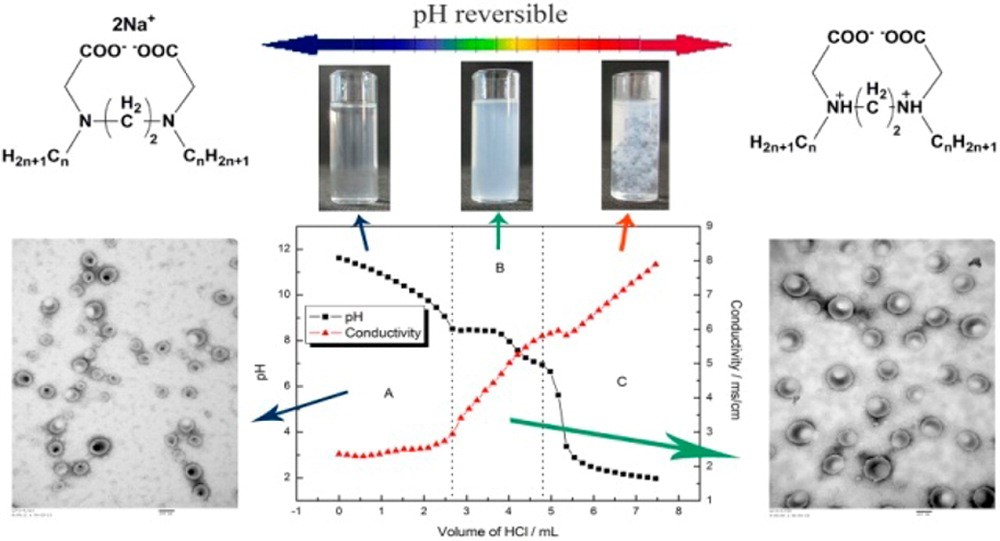
\includegraphics[width=.75\textwidth]{figure/switchable-ph.jpg}\\
        \caption{pH开关表面活性剂控制的乳液类型转变\cite{lv2014}}
        \label{fig:switchable-ph}
    \end{figure}

    除通过pH调节表面活性剂的亲疏水性改变体系性质外,Brazdova\cite{李云霞2011,brazdova2008}等
    制得氨基环己醇衍生脂质体表面活性剂,通过 pH 控制分子构象作为开关,见图\ref{fig:switchable-ph-conformation}。
    \begin{figure}[htbp]
        \centering
        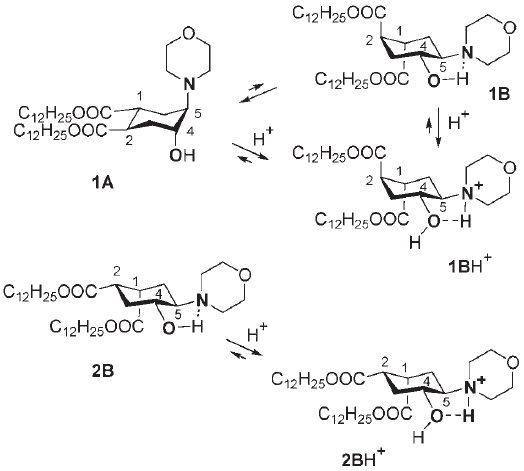
\includegraphics[width=.5\textwidth]{figure/switchable-ph-conformation.png}\\
        \caption{pH 触发的氨基环己醇衍生脂质构象变化\cite{brazdova2008}}
        \label{fig:switchable-ph-conformation}
    \end{figure}

    \subsection*{(5) \ce{CO2}/\ce{N2}开关表面活性剂}
    \ce{CO2}型开关表面活性剂其作用原理在本质上和酸碱开关表面活性剂类似,利用 \ce{CO2}
    气体的弱酸性,随着 \ce{CO2}的通入和排出,体系的 pH 发生变化,从而引起体系内可离子化基团的
    质子化或去质子化,导致表面活性剂亲疏水性发生变化,进而影响体系的表面活性。迄今为止,
    \ce{CO2}开关型表面活性剂主要包括脒/\ce{CO2}体系、胍/\ce{CO2}体系以及胺/\ce{CO2}体系\cite{梅平2016}。
    
    \ce{CO2}型开关表面活性剂采用 \ce{CO2}作为调控手段,相比其他调控手段而言,具有价格便宜、
    无毒无害且易于脱除等优点\cite{jessop2012},可应用于重油输送、土壤清洗、油砂分离及乳化
    聚合\cite{jessop2012}。同可分解表面活性剂一样,早在开关表面活性剂概念提出之前,\ce{CO2}型
    开关表面活性剂已投入使用,Moore 和 Lefevre 采用 \ce{CO2}作为丁二烯/苯乙烯乳液聚合的开关表面
    活性剂,见图\ref{fig:switchable-co2-a},其中式左化合物具有乳化作用而式右化合物不具有乳化作用。
    \begin{figure}
    \centering
        \begin{subfigure}[b]{\textwidth}
            \centering
            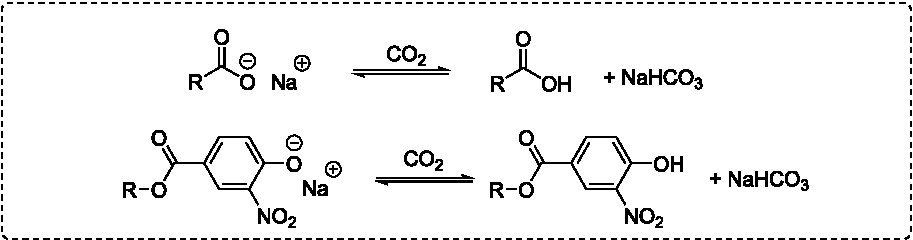
\includegraphics[scale=0.8]{Figure/switchable-co2-a.pdf}
            \caption{Moore和Lefevre采用的丁二烯/苯乙烯乳液聚合可调控乳化剂}\label{fig:switchable-co2-a}
        \end{subfigure}%
    
        \begin{subfigure}[b]{\textwidth}
            \centering
            
\includegraphics[scale=0.8]{Figure/switchable-co2-b.pdf}
            \caption{Jessop课题组提出的 \ce{CO2}开关表面活性剂}\label{fig:switchable-co2-b}
        \end{subfigure}%
    \caption{早期应用及研究的 \ce{CO2}型开关表面活性剂}
    \label{fig:switchable-co2}
    \end{figure}
    
    2006年,Jessop课题组\cite{liu2006science}提出一类脒类化合物可用 于\ce{CO2}开关表面活性剂,
    见图\ref{fig:switchable-co2-b}。此外,三级胺也可用于 \ce{CO2}开关表面活性剂,但一级、二级胺
    则因为形成氨基甲酸酯在开关表面活性剂应用中有所难度\cite{jessop2012}。
    
    \subsection*{(6) 氧化还原开关表面活性剂}
    氧化还原型开关表面活性剂主要采用电化学方法或化学手段改变表面活性剂分子结构,从而达到
    调整表面活性的目的。其中,前者研究最早且较为成熟的是二茂铁基表面活性剂,其包含阳离子-两性离子
    可逆转换和阴离子-两性离子可逆转换两类\cite{李云霞2011}。图\ref{fig:switchable-redox-cp2fe}中前者是
    一类二茂铁基表面活性剂。但二茂铁基开关表面活性剂所需使用的二茂铁基团价格对该类表面活性剂的广泛
    使用有所限制,同时也存在需要添加电解质和反应时间长的问题。
    \begin{figure}[htbp]
        \centering
        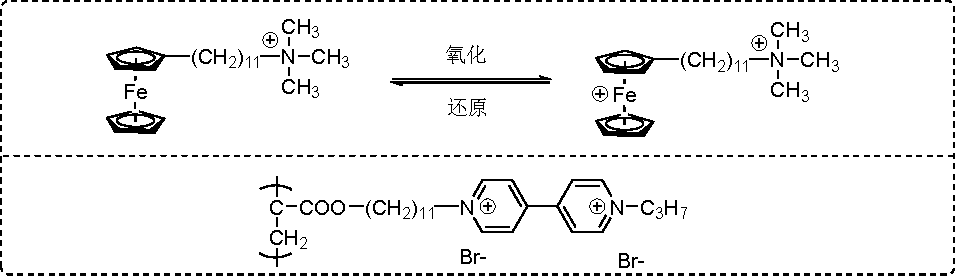
\includegraphics[scale=0.8]{Figure/switchable-cp2fe.pdf}\\
        \caption{电化学方法实现 的氧化还原开关表面活性剂}\label{fig:switchable-redox-cp2fe}
    \end{figure}
    
    此外,甲基紫类结构,即联吡啶类结构(图\ref{fig:switchable-redox-cp2fe})的表面活性剂也是一类良好的
    氧化还原型开关表面活性剂,其毒性较高,如氯化二甲基联吡啶(即百草枯主要成分,一种高毒植物农药)。
    
    除电化学方法实现的氧化还原开关表面活性剂外,含二硫键结构的表面活性剂可在含巯基试剂作用下断裂,
    从而改变分子结构。2008年,Fan等\cite{fan2008}合成一种含二硫键的氨基酸型双子表面活性剂
    (图\ref{fig:switchable-redox-disulfide}),在二硫苏糖醇 (DTT) 作为还原剂和 \ce{H2O2} 作为氧化剂的作用
    下,可以实现双子表面活性剂和单链表面活性剂之间的转变。
    \begin{figure}[htbp]
        \centering
        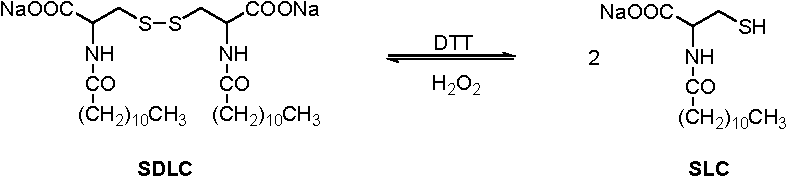
\includegraphics[scale=0.8]{figure/switchable-disulfide.pdf}\\
        \caption{SDLS/SLC的氧化还原反应\cite{fan2008}}\label{fig:switchable-redox-disulfide}
    \end{figure}
    
    此外,对于刺激响应性表面活性剂,还存在电解质以及酶等刺激手段,例如离子型表面活性剂对溶液中的
    离子强度敏感,一些表面活性剂在酶催化下可催化分解,如氯化肉豆蔻酰胆碱在丁酰胆碱酯酶作用酯键断裂\cite{guo2012},
    这些均属于刺激响应性表面活性剂。
    
%    最后,含硒表面活性剂作为一种新型的氧化-还原开关表面活性剂,Kong等\cite{kong2016redox}利用
%    \ce{H2O2}将硒醚氧化为硒亚砜,使尾链亲水性增加,且在\ce{Na2SO3}等还原条件下又可恢复原结构。
%    
%    图 13 含硒氧化-还原表面活性剂的可逆转化\cite{kong2016redox}
    
%    \subsection*{(7) 酶开关表面活性剂}
%    除以上类型的开关表面活性剂之外,还有酶催化\cite{ku2011}
%【Enzyme-triggered model self-assembly in surfactant–cyclodextrin systems】的开关表面活性剂有待讨论。
    
    \section{含硒表面活性剂}
    含硒表面活性剂是一类新型的氧化还原型开关表面活性剂,2010年Zhang Xi等\cite{zhangxi2010,zhangxi20102}
    首次报道了一种含硒阳离子表面活性剂,利用其与具有羧酸根的两亲嵌段共聚物进行自组装,形成具有
    氧化响应性的胶束,之后该课题组报道了多例利用含硒表面活性剂实现的具有氧化还原刺激响应性的胶束体系,
    硒原子分别位于两亲嵌段共聚物内部和侧链。
    
    2015年Liu X F等\cite{zhang2015}报道了含硒磺基甜菜碱类表面活性剂,将其与十二烷基硫酸钠复配,
    形成了具有氧化还原响应的蠕虫状胶束体系,通过氧化还原反应可使表面活性剂可逆地在硒醚和硒亚砜
    (\ce{Se=O})之间变化,从而使体系在蠕虫状胶束个囊泡之间切换。
    
    2016年Liu X F等\cite{zhang2016}等使用十二烷基亚硒酸钾制备了乳液,在酸性条件下十二烷基亚硒酸可被KI
    还原为双十二烷基二硒醚,从而失去乳化作用,溶液分层;在碱性条件下,二硒醚可被 \ce{I2}氧化为亚硒酸,
    从而体系恢复为乳液,见图\ref{fig:switchable-selenium}。 
    \begin{figure}[htbp]
        \centering
        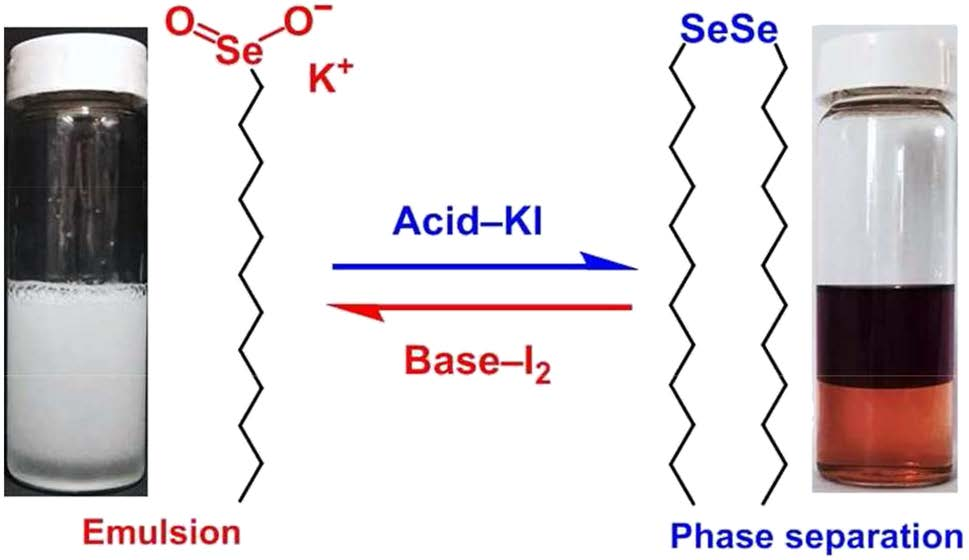
\includegraphics[scale=0.8]{figure/switchable-selenium.jpg}\\
        \caption{含硒表面活性剂控制的氧化还原刺激响应乳液\cite{zhang2016}}\label{fig:switchable-selenium}
    \end{figure}

    \section{囊泡}
    囊泡是一种由表面活性剂双分子层闭合而成的聚集体。双分子层内壁和外壁均为
    亲水头基,内腔充满水相,疏水尾链则被包裹在双分子层内部(反相囊泡在有机相中形成,其双分子层
    恰好翻转),囊泡一般是由这样的一层或多层双分子层闭合而成,一般具有球形结构,此外还有椭球形、
    扁球形等。
    
    囊泡是表面活性剂分子构成的聚集体结构中的一种,按照 Israelachvili 和 Mitchell 等人提出的临界堆积参数
    理论 (critical packing parameter theory),可以通过表面活性剂分子的几何形状对其在水溶液中的聚集体进行预测:
    \begin{equation}\label{eq:cpp}
        p=\frac{\upsilon}{al}
    \end{equation}
    
    式\ref{eq:cpp}中,$p$为临界堆积参数,$a$为亲水头基平均占据横截面积,$l$为疏水链平均链长,$\upsilon$
    为疏水链的体积。当$p<1/3$时一般形成球状胶束或不连续的立方相;当$1/3<p<1/2$时易形成椭球形或棒状
    胶束;当$1/2<p<1$时可形成囊泡、碟形胶束或层状相等不同曲率的双分子层结构;当$p>1$时会形成反相
    结构,见图\ref{fig:scheme-cpp}所示。
    \begin{figure}[htbp]
        \centering
        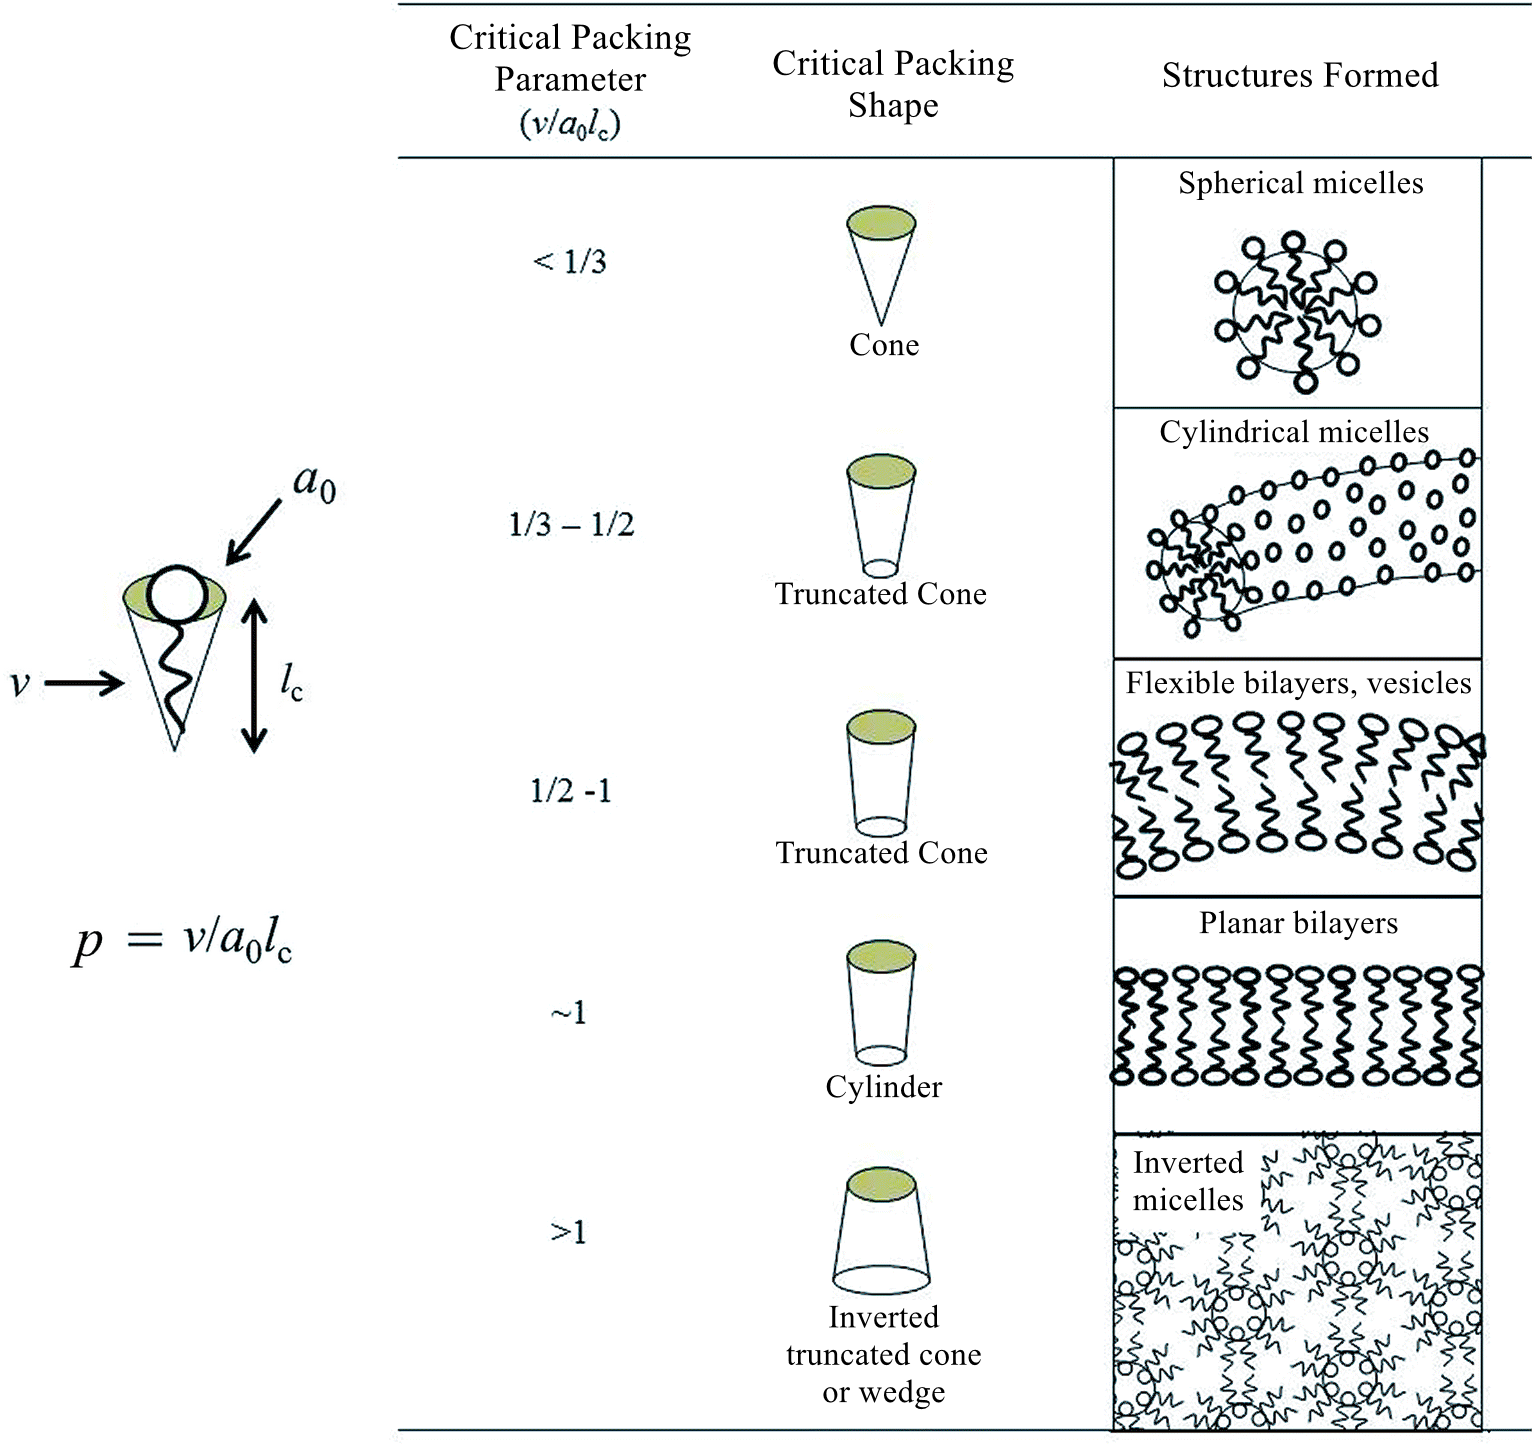
\includegraphics[width= .826\textwidth]{figure/scheme-cpp.png}\\
        \caption{临界堆积参数理论预测的表面活性剂聚集体形态\cite{salim2014}}\label{fig:scheme-cpp}
    \end{figure}

    其中,对碳氢链为直链的表面活性剂分子,$\upsilon$和$l$可按Tanford方程计算:
    \begin{align}\label{eq:cpp2}
        \upsilon &= 27.4+26.9n\\
        l &= 1.5+1.265n
    \end{align}
    式\ref{eq:cpp2}中$n$为疏水碳链碳原子数。
    
    大多表面活性剂分子的$p$值均小于$1/3$,故通常情况它们只能构成球状胶束;对于双链表面活性剂
    而言,如双(2-乙基己基)琥珀酸磺酸钠 (AOT),其疏水基团增大,$p$值可位于$1/2$-$1$之间,则或可形成
    囊泡或双层结构\cite{翟利民2007} 。现将单链阴阳离子表面活性剂进行复配,则带电头基之间的静电
    作用可使阴阳离子表面活性剂形成拟双子结构,这样一来也增加了疏水结构体积,或可形成囊泡结构。
    
    囊泡显著区别于胶束等聚集体结构的一个特征是,具有囊泡结构的溶液在外观上呈现淡蓝色,并且囊泡属于
    各向异性的相,在偏光片下呈现双折射纹理,在显微镜中通常能够观察到马耳他十字花\cite{刘洪国2016}。
        
    \subsection{囊泡的制备方法}
    脂质体是发现和研究最早的囊泡体系,所不同的是其双分子层为磷脂双分子层,Stoeckenius在1959年将磷脂
    在水中溶胀得到多层结构\cite{刘洪国2016},后被证明是闭合的双分子层结构。目前所说的囊泡一般指由表面
    活性剂分子构成,早期构筑囊泡常需要借助外力,如采用溶胀法、乙醚注射法、超声分散法、挤压法等,但是
    这些由外力制备的囊泡通常不稳定,所制备的囊泡容易解体\cite{刘洪国2016}。
    
    20世纪80年代出,人们开始关注于囊泡的自发形成,1983年Ninham等人\cite{ninham1983}发现双十二烷基
    二甲基氢氧化铵 (DDAOH) 可以自发形成囊泡并且相当稳定,随后发现双十二烷基二甲基铵盐也可以自发形成
    囊泡。1989年Kaler等\cite{kaler1989}发现阴阳离子表面活性剂十二烷基苯磺酸钠 (SDBS) 和十六烷基三甲基
    对甲苯磺酸盐 (CTAT) 的混合体系能够形成自发囊泡,这打破了以往“阴阳离子表面活性剂因混合产生沉淀而
    不能混合使用”的观念,但是Kaler的研究体系中当阴阳离子表面活性剂浓度较高、链长相近或接近等摩尔量
    混合时依然产生沉淀,见图\ref{fig:vesicle-phase}。    
    \begin{figure}[htbp]
        \centering
        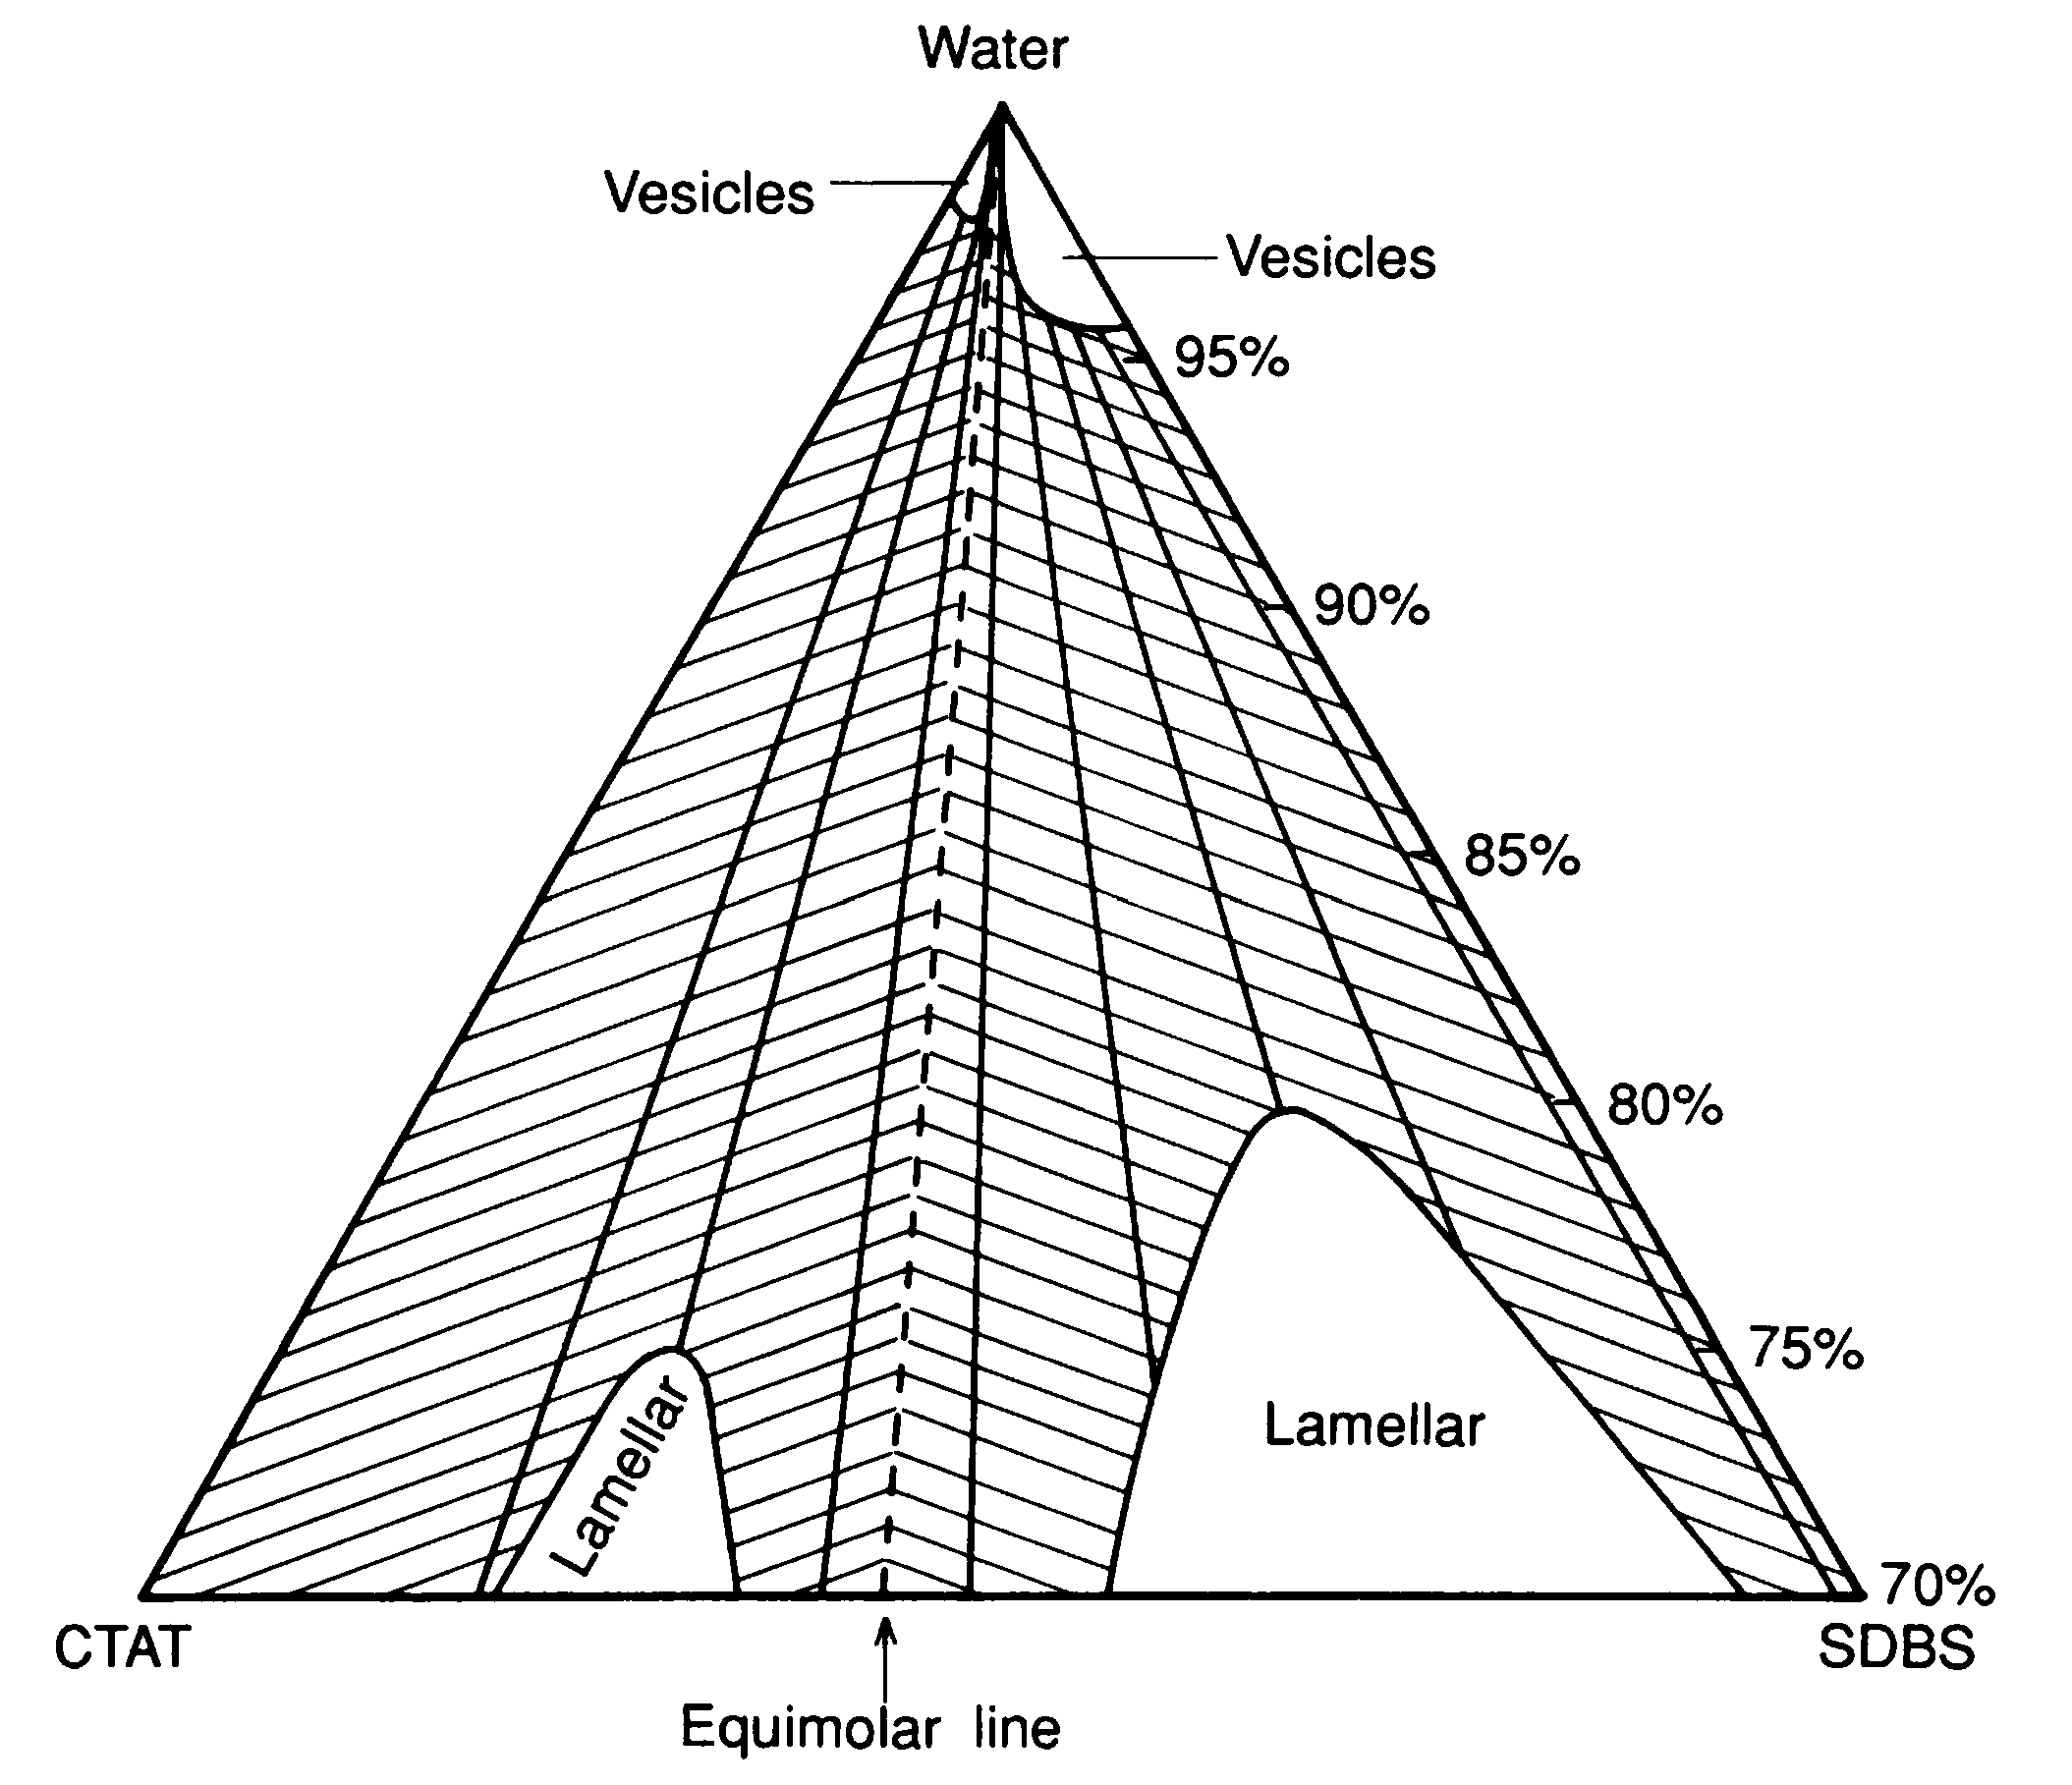
\includegraphics[width= .475\textwidth]{figure/vesicle-phase.png}\\
        \caption{阴阳离子表面活性剂SDBS和CTAT混合体系的相图\cite{kaler1989}\\{\footnotesize{(阴影区域代表沉淀)}}}
        \label{fig:vesicle-phase}
    \end{figure}

    一般认为,阴阳离子复配体系中囊泡相的形成是由于形成的阴/阳离子对降低可表面活性剂亲水头基的有效
    截面积所导致的\cite{刘洪国2016}。但同时也因为阴/阳离子对的形成造成聚集体表面电荷密度下降,从而使得
    在接近等摩尔量混合时体系不稳定,产生沉淀。
    
    除阴阳离子表面活性剂复配体系外,嵌段共聚物、糖酯类分子、小分子表面活性剂体系如双尾链的阳离子表面
    活性剂、高价金属离子表面活性剂/长链烷基氢氧化铵复配体系和脂肪酸及其助表面活性剂等体系中也可自发
    形成囊泡\cite{刘洪国2016}。
        
    \subsection{囊泡的应用}
    囊泡可因其结构独特可用于生物膜模拟、软模板或微反应器、药物装载和靶向释放以及毛细管电动色谱等
    领域\cite{蒋玲玲2018}。
    
    囊泡因其结构独特,可提供多种微环境包括水相空腔、疏水双分子层以及囊泡外表面,限制客体物质在溶液
    中的位置并诱导材料的和合成和组装,可用于合成微纳米材料,并且聚集体模板的脱除对材料的形貌几乎
    没有损伤。
    
    药物载体可以起到改变药物在体内分布并具有靶向释放作用。脂质体是研究最多的靶向药物载体,多用于
    抗肿瘤药物,但其存在着化学不稳定、原料难以纯化、包封率不高容易泄漏等缺点。合成表面活性剂形成
    的囊泡相对脂质体更加稳定。存在研究表明人体病变部位活性氧水平会显著升高,因此能够具有活性氧
    物种刺激响应性的药物载体能够达到靶向释放的作用,图\ref{fig:vesicle-ros}中的多种具有活性氧物种
    响应性结构可用于设计刺激响应性药物载体。
    \begin{figure}[htbp]
        \centering
        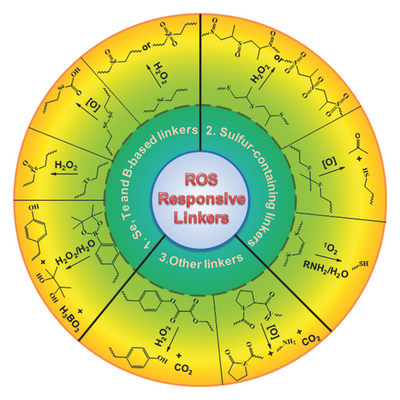
\includegraphics[width= .426\textwidth]{figure/vesicle-ros.png}\\
        \caption{用于活性氧物种刺激响应性药物载体设计的代表性结构\cite{saravanakumar2017}}
        \label{fig:vesicle-ros}
    \end{figure}
    
    \section{立题依据和研究内容}
    \subsection{立题依据}
    开关表面活性剂及其自组装体系的智能响应行为是目前国内外学界普遍关注的问题,
    而含硒表面活性剂的氧化还原响应灵敏、条件温和,在生命领域具有重要的应用前景;
    表面活性剂囊泡分子量相对较小,合成较为简单,受到外界刺激时反应较为迅速,
    复配时容易自发聚集生成稳定的囊泡。结合两者的优点,考虑通过氧化还原响应来控制
    含硒表面活性剂胶束和囊泡之间的转换,基于氧化还原刺激响应性囊泡在作为药物控制
    递送载体、微反应器、合成中空颗粒模板等领域有着很大的期许效用。
    
    \subsection{研究内容}
    本论文着重进行了含硒表面活性剂囊泡的构筑及其性质研究。主要研究内容如下:
    \begin{enumerate}
        \item 合成两种含硒阴离子表面活性剂,提纯并表征确认其结构;
        \item 提纯与阴离子表面活性剂复配的阳离子表面活性剂,将阴阳离子表面活性剂
        按不同摩尔比进行复配以构筑囊泡,采用动态光散射测试复配体系中的聚集体粒径;
        \item 测试复配体系耐盐效果,选定复配囊泡体系,测试囊泡粒径随时间的变化关系,
        考察囊泡的稳定性;
        \item 配置不同浓度的表面活性剂复配体系,测试其中囊泡的粒径变化关系;
        \item 对囊泡体系进行氧化还原测试,考察其氧化还原响应性,包含氧化、还原所需
        时间;对还原后的体系进行粒径测试,探究与初试状态的变化;进行多次氧化还原
        循环,考察体系的刺激响应耐受性;
        \item 对两种含硒表面活性剂的复配囊泡体系的性质进行对比。
    \end{enumerate}
    
    %%%%%%%%%%%%%%%%%%%%%%%%%%%%%%%%%%%%%%%%%%%%%%%%%%%%%%%%%%%%%%%%%%%%%%%%%%%%%%%
    \chapter{实验部分}\label{chapter:experiment}
    \section{实验仪器与试剂}
        \begin{table}[htp]
        \centering
        \begin{tabular}{ccc}
            \toprule
            \textbf{仪器/试剂} & \textbf{规格/型号} & \textbf{生产厂家} \\
            \midrule
            硒   & GR & 阿达玛斯试剂 \\
            硼氢化钠  & AR  & 上海化学试剂有限公司 \\
            1-溴代十二烷
            1-溴代丁烷  & CP & 国药集团化学试剂有限公司 \\
            3-溴丙醇 & GR & 阿达玛斯试剂 \\
            11-溴-1-十一醇 & GR & 阿达玛斯试剂 \\
            氯磺酸  & CP & 上海化学试剂有限公司 \\
            碳酸钠  & AR & 国药集团化学试剂有限公司 \\
            十二烷基三甲基溴化铵 & CP & 国药集团化学试剂有限公司\\
            30\%过氧化氢  & AR & 上海化学试剂有限公司 \\
            亚硫酸钠  & AR & 国药集团化学试剂有限公司 \\
            硫酸钠  & AR & 国药集团化学试剂有限公司 \\
            超纯水 & Simplicity\ce{^{\textregistered}} UV & 美国Merck Millipore\\
            电子分析天平  & JY2015 & 梅特勒-托利多有限公司 \\
            旋转蒸发器  & RE-2000B & 上海亚荣生化仪器厂 \\
            超声波清洗器  & KQ-100B & 昆山市超声仪器有限公司 \\
            超级恒温水浴  & CS501 & 上海博迅实业有限公司 \\
            核磁共振谱仪  & AVANCE Ⅲ HD 400MHz & 瑞士布鲁克公司 \\
            液相色谱质谱联用仪  & LCZ/2690 XE/996 & 美国沃特世公司 \\
            激光光散射仪 & ALV/DLS/SLS-5022F & 德国ALV公司\\
            \bottomrule
        \end{tabular}
        \caption{实验仪器与试剂}\label{table:实验仪器与试剂}
    \end{table}
    
    \section{含硒表面活性剂的制备}
    \subsection{合成路线}
    按图\ref{fig:scheme-synthesis}所示合成路线制备两种含硒表面活性剂3-十二烷基硒-1-丙基硫酸钠 
    (5a, SDSePS) 和11-丁基硒-1-十一烷基硫酸钠 (5b, SBSeUS)。
    \begin{figure}[htbp]
        \centering
        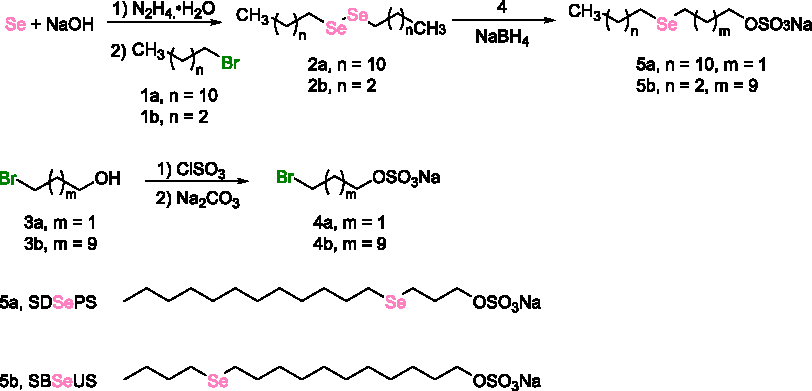
\includegraphics[scale=1]{figure/scheme-synthesis.pdf}\\
        \caption{含硒表面活性剂的合成路线}\label{fig:scheme-synthesis}
    \end{figure}

    \subsection{实验方法}
    \subsection*{A. SDSePS的制备}
    \paragraph*{(1) 对称二硒醚的制备}
    称取 9.28 g (0.12 mol) 硒粉于 500 mL 三口圆底烧瓶中,加入 6.40 g (0.16 mol) NaOH;冰浴条件下
    缓慢加入2.50 g (0.05 mol) \ce{N2H4.H2O},反应过程采用 \ce{N2}保护,反应至体系呈棕红色; 
    滴加 140 mL 四氢呋喃 (THF) 溶解的 29.31 g (0.12 mol) \ce{C12H25Br} (1a),50 ℃下反应 18 h后停止
    反应。
    
    对反应后的混合液采用二氯甲烷(\ce{CH2Cl2})萃取分液,用无水 \ce{Na2SO4}干燥后减压抽滤、减压旋干
    溶剂,乙酸乙酯热溶后重结晶三次,真空干燥 12 h,得 20.41 g 黄色针状产物2a,得率 71.60\%。
    
    \paragraph*{(2) 卤代醇的磺化}
    称取 20 g (0.14 mol) \ce{Br(CH2)3OH} (3a) 置于 500 mL 四口圆底烧瓶中,加入 150 mL 干燥 \ce{CH2Cl2},
    冰浴条件下搅拌 10 min,缓慢滴加 19.5 g (0.17 mol) 氯磺酸(\ce{ClSO3H}),室温下反应 30 min后用
    饱和 \ce{Na2CO3}水溶液中和,调节 pH 8-9。
    
    停止反应后,减压旋干溶剂,无水乙醇热溶除盐,乙醇重结晶三次后真空干燥 12 h,得 24.04 g 白色产物
    4a,得率 71.25\%。
    
    \paragraph*{(3) 阴离子表面活性剂的制备}
    称取 15 g (0.03 mol) 对称二硒醚2a置于 500 mL 三口圆底烧瓶中,加入 150 mL 四氢呋喃充分搅拌,反应
    过程 \ce{N2} 保护,冰浴条件下缓慢滴加 100 mL 去离子水溶解的 5.67 g (0.15 mol) \ce{NaBH4}至体系
    逐渐变白,然后室温反应 20 min,再滴加 100 mL 去离子水溶解的 16 g (0.66 mol) 溴代烷基硫酸钠4a,
    室温反应 24 h。
    
    停止反应后,减压旋干溶剂,无水乙醇热溶除盐,以体积比乙酸乙酯:甲醇 = 5:1 为洗脱剂柱色谱
    分离,后采用无水乙醇重结晶,得 18.6 g 产物5a,得率 75.80\%。
    \subsection*{B. SBSeUS的制备}
    称取15.82 g (0.20 mol) 硒粉于500 mL 三口烧瓶内,加入 9.88 g (0.24 mol) NaOH;冰浴条件加入四氢呋喃 (THF)
    100 mL;称取 3.81 g (0.32 mol) \ce{N2H4.H2O} (85 wt. \%) 于滴液漏斗中,缓慢滴加入三口烧瓶,瓶内黑色物质
    变为红褐色粘稠状;待上层液体由浑浊变为澄清,缓慢滴加28.6 g (0.21 mol) \ce{C4H9Br} (THF溶解),25 ℃下反应12 h,
    反应过程采用 \ce{N2} 保护。
    
    反应后混合液减压抽滤,得澄清黄色液体,减压旋干溶剂;加入\ce{CH2Cl2},采用 \ce{H2O} 萃取 NaBr三到四次,
    用无水 \ce{Na2SO4} 干燥后减压抽滤,减压除去 \ce{CH2Cl2} 和 \ce{H2O}。
    
    SBSeUS (5b)的后续步骤后处理方法与SDSePS (5a)的制备方法相同。
    
    \subsection{表征方法}
    对所制备的含硒阴离子表面活性剂采用 \ce{CD3OD}为溶剂进行核磁氢谱测试,以 \ce{CH3OH}作为溶剂采用
    液相色谱质谱联用仪进行质谱测试,以确认所得化学物是否为目标化合物。
    
    \section{复配囊泡的构筑}
    \subsection*{(1) DTAB的纯化}
    以无水乙醇和乙酸乙酯作为溶剂,在50 ℃下对十二烷基三甲基溴化铵 (DTAB) 进行重结晶提纯,提纯两次,
    真空干燥后,密封保存备用。
    
    \subsection*{(2) 阴阳离子表面活性剂复配}
    使用实验室自制超纯水分别配置一定体积的5 mmol/L和10 mmol/L的阳离子表面活性剂DTAB水溶液,
    同样方法配置5 mmol/L和10 mmol/L含硒阴离子表面活性剂SDSePS和SBSeUS水溶液,然后使用 0.22 $\mu$m 的水系滤膜
    对上述溶液进行过滤作为母液备用。
    
    将阴离子和阳离子表面活性剂以不同摩尔比 (1:9、2:8、3:7、4:6、5:5、6:4、7:3、8:2、9:1)复配为5 mL溶液于洁净
    无尘的动态光散射样品瓶内,即使用上述母液按体积比混合,超声振荡后,置于30 ℃水浴中恒温12 h后进行后续测试。
        
    \section{囊泡的性质研究}
    \subsection{阴阳离子表面活性剂不同摩尔比的影响}
    使用上述母液按不同摩尔比 (1:9、2:8、3:7、4:6、5:5、6:4、7:3、8:2、9:1) 配置不同摩尔比的阴阳离子表面活性剂
    复配体系,混合液体积均为5 mL,放置于洁净无尘的动态光散射样品瓶内,置于30 ℃水浴中恒温12 h。
    
    12 h后记录不同摩尔比复配体系的外观现象,后采用ALV/DLS/SLS-5022F型激光光散射仪在30 ℃测试所有体系内的
    聚集体粒径,该仪器采用He-Ne激光发射器作为光源,发射波长633 nm,散射角$90^\circ$,使用累计法分析强度自相关
    函数。
    
    \subsection{复配体系的稳定性}
    从耐盐性和对时间稳定性两个方面考察复配体系的稳定性。
    
    采用 \ce{Na2SO4}测试复配体系的耐盐状况,以少量多次的方式向复配体系中加入 \ce{Na2SO4}直至体系发生囊泡消失
    或沉淀等新相变化。采用 \ce{Na2SO4}进行耐盐性测试,是由于在氧化还原刺激响应性过程中,会存在副产物 \ce{Na2SO4} 
    的产生。
    
    使用动态光散射对阴阳离子表面活性剂复配囊泡体系中的聚集体粒径进行测试,连续跟踪粒径变化10天。
    
    \subsection{不同浓度对复配体系的影响}
    使用上述5 mmol/L、10 mmol/L的母液进行稀释,可得到0.5 mmol/L、1 mmol/L、2 mmol/L、2.5 mmol/L、
    5 mmol/L、10 mmol/L的阴阳离子表面活性剂溶液。根据先前的实验结果选定一个最佳的摩尔配比,按此摩尔比
    配置不同浓度的复配囊泡体系,对复配体系在30 ℃下恒温静置12 h,记录外观现象后采用激光光散射仪测试
    所有复配体系中的聚集体存在情况。
    
    \subsection{复配体系的氧化还原刺激响应性能}
    采用 \ce{H2O2}作为氧化剂、\ce{Na2SO3}作为还原剂考察复配体系的氧化还原刺激响应性能。
    
    由于含硒阴离子表面活性剂分子中的硒原子可被可逆的氧化和还原,初步采用1.2倍相当于复配体系中阴离子表面活性剂
    的量的 \ce{H2O2} 对复配体系进行氧化,使用薄层色谱监测是否氧化完全,记录氧化完成时间及氧化后的体系外观现象,
    对氧化后的体系使用激光光散射仪进行动态光散射测试其中的聚集体状况。
    
    向氧化过后的体系加入与 \ce{H2O2} 相同量的 \ce{Na2SO3} 进行还原,采用薄层色谱监测还原过程,使用动态光散射
    测试还原后的体系中聚集体粒径变化。
    
    按上述操作对复配体系进行多次氧化还原过程,考察体系的氧化还原刺激响应性能。
    
   %%%%%%%%%%%%%%%%%%%%%%%%%%%%%%%%%%%%%%%%%%%%%%%%%%%%%%%
    \chapter{实验结果与讨论}\label{chapter:results}
    \section{含硒表面活性剂的表征与分析}
    \subsection{SDSePS的结构表征与分析}
    以 \ce{CD3OD}为溶剂,对纯化后的样品进行 \ce{^1H} NMR 表征,表征结果如图\ref{fig:SDSePS-nmr}所示。
    \begin{figure}[htbp]
        \centering
        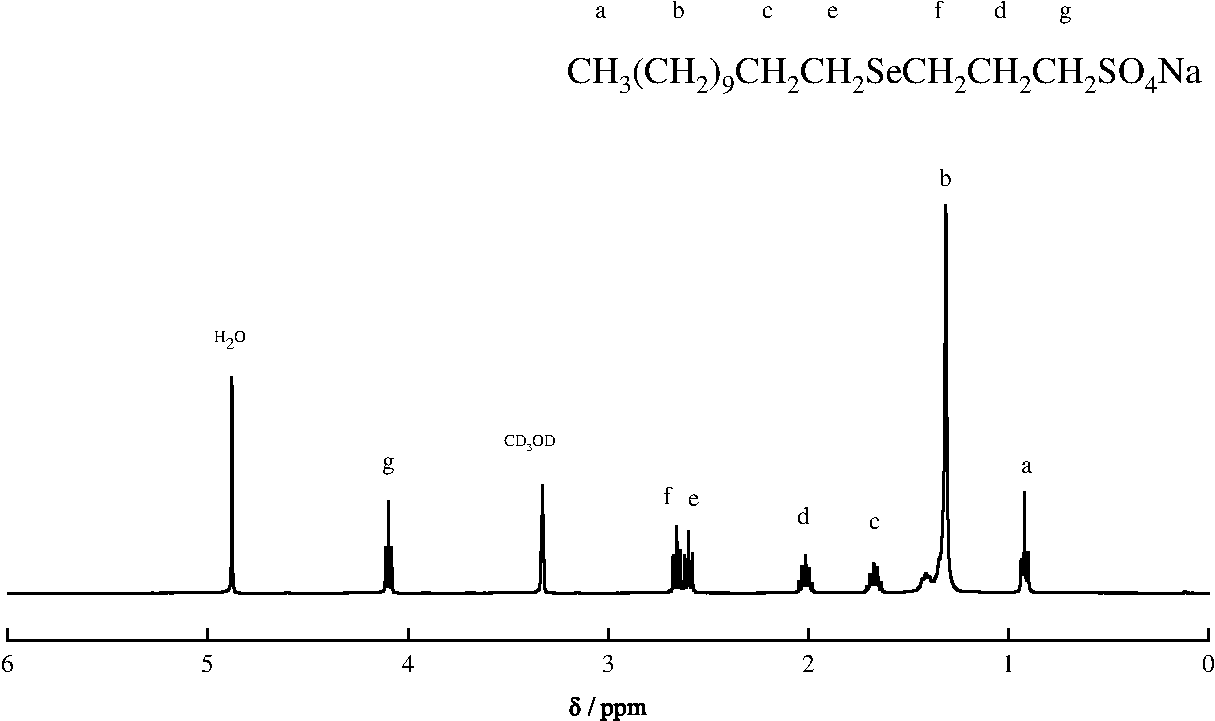
\includegraphics[width=.7\textwidth]{figure/SDSePS-nmr.pdf}\\
        \caption{SDSePS的核磁氢谱}\label{fig:SDSePS-nmr}
    \end{figure}
     
    \ce{^1H} NMR (400 MHz, \ce{CD3OD}, 图\ref{fig:SDSePS-nmr}) δ 0.92 (t, \textit{J}=8.0 Hz, 3H), 1.31-1.41 (overlap, 18H), 
    1.67 (m, 2H), 2.01 (m, 2H), 2.60 (t, \textit{J}=8.0 Hz, 2H), 2.66 (t, \textit{J}=8.0 Hz, 2H),  4.10 (t, \textit{J}=6.0 Hz, 2H).
    
    对SDSePS的核磁共振氢谱进行解析,图\ref{fig:SDSePS-nmr}中,$\delta$ = 3.30的峰为 \ce{CD3OD}溶剂残留峰,
    $\delta$ = 4.87为水峰\cite{波谱解析} ,峰a为 SDSePS 疏水链端甲基的氢信号,以其积分个数为 3 计算,
    实际总氢个数为 31.68,理论氢个数为 31,氢个数基本吻合;峰b为长碳链出峰,氢个数为18;峰c、d分别为Se的两端
    $\beta$位亚甲基氢出峰\cite{徐辉碧1994,reich1978},其中峰d更靠近极性头基(\ce{-SO4^-})向低场移动;峰e、f分别为Se的两端$\alpha$位亚甲基氢出峰;
    $\delta$ = 4.10处峰g为靠近极性头基(\ce{-SO4^-})的亚甲基氢出峰。各峰化学位移与氢个数均可与目标产物对应,
    由此推断所测样品即为目标产物。
    
    以 \ce{CH3OH}为溶剂,对SDSePS采用负离子模式进行 ESI-MS 测试,测试结果如图\ref{fig:SDSePS-mass}所示。
     \begin{figure}[htbp]
        \centering
        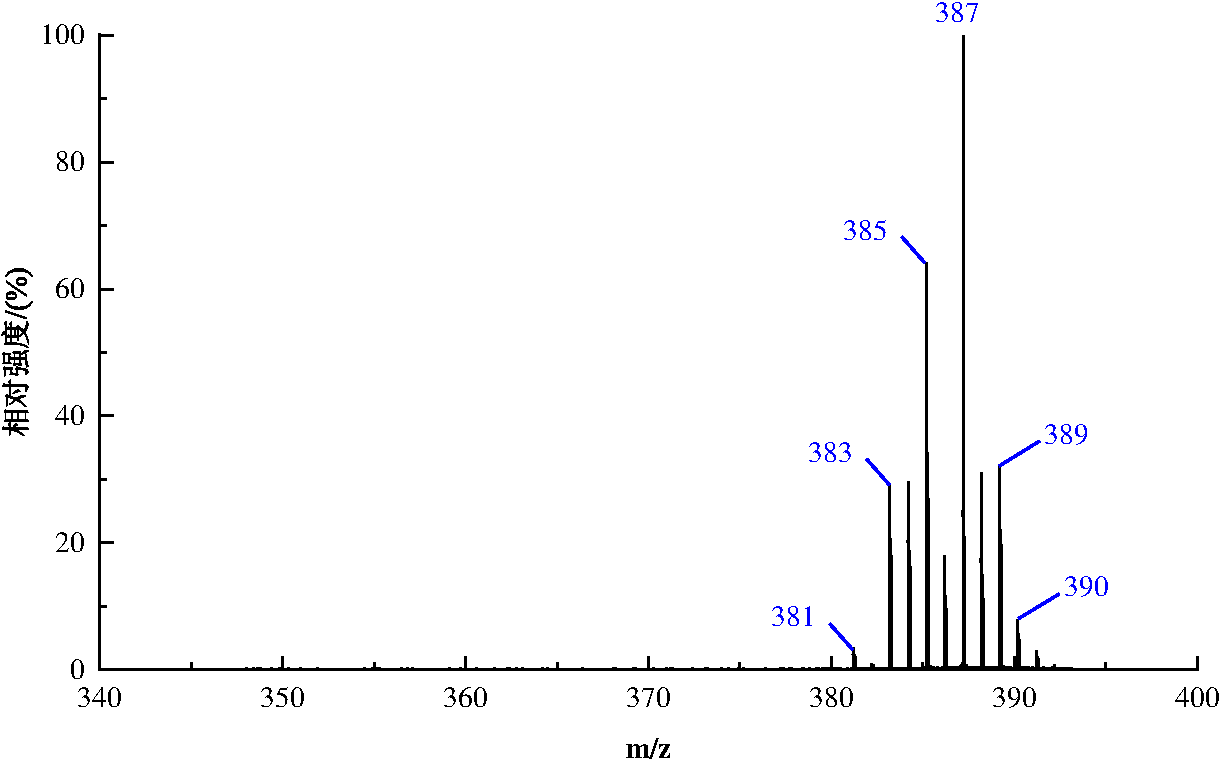
\includegraphics[width=.7\textwidth]{figure/SDSePS-mass.pdf}\\
        \caption{SDSePS的质谱}\label{fig:SDSePS-mass}
    \end{figure}
    
    负离子模式下,相对强度最高的$m/z = 387$的峰应为 \ce{C12H25SeC3H6SO4-}的分子离子峰,与 \ce{C15H31SO4Se}
    的计算结果386.42基本相符,同时硒有多种稳定的同位素,\ce{^74Se} (0.87\%)、\ce{^76Se} (9.02\%)、\ce{^77Se} (7.58\%)、
    \ce{^78Se} (23.52\%)、\ce{^80Se} (49.82\%)、\ce{^82Se} (9.19\%),也与测试结果相符合。
%    \begin{figure}[htbp]
%    \centering
%        \begin{subfigure}[b]{.475\textwidth}
%            \centering
%            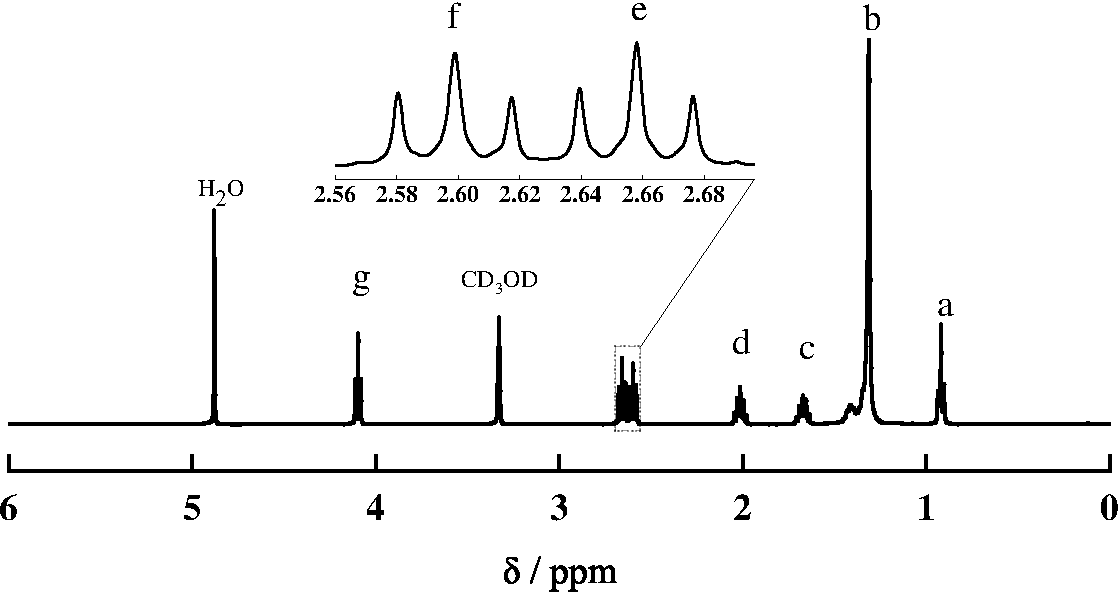
\includegraphics[width=\textwidth]{figure/nmr123.pdf}
%            \caption{核磁}\label{}
%        \end{subfigure}
%        \hfill
%        \begin{subfigure}[b]{.475\textwidth}
%            \centering
%            \includegraphics[width=\textwidth]{example-image}
%            \caption{质谱}\label{}
%        \end{subfigure}
%    \caption{12+3结构表征}\label{fig:cleavable-saa}
%    \end{figure}
    
    \subsection{SBSeUS的结构表征与分析}
        以 \ce{CD3OD}为溶剂,对纯化后的样品进行 \ce{^1H} NMR 表征,表征结果如图\ref{fig:SBSeUS-nmr}所示。
    \begin{figure}[htbp]
        \centering
        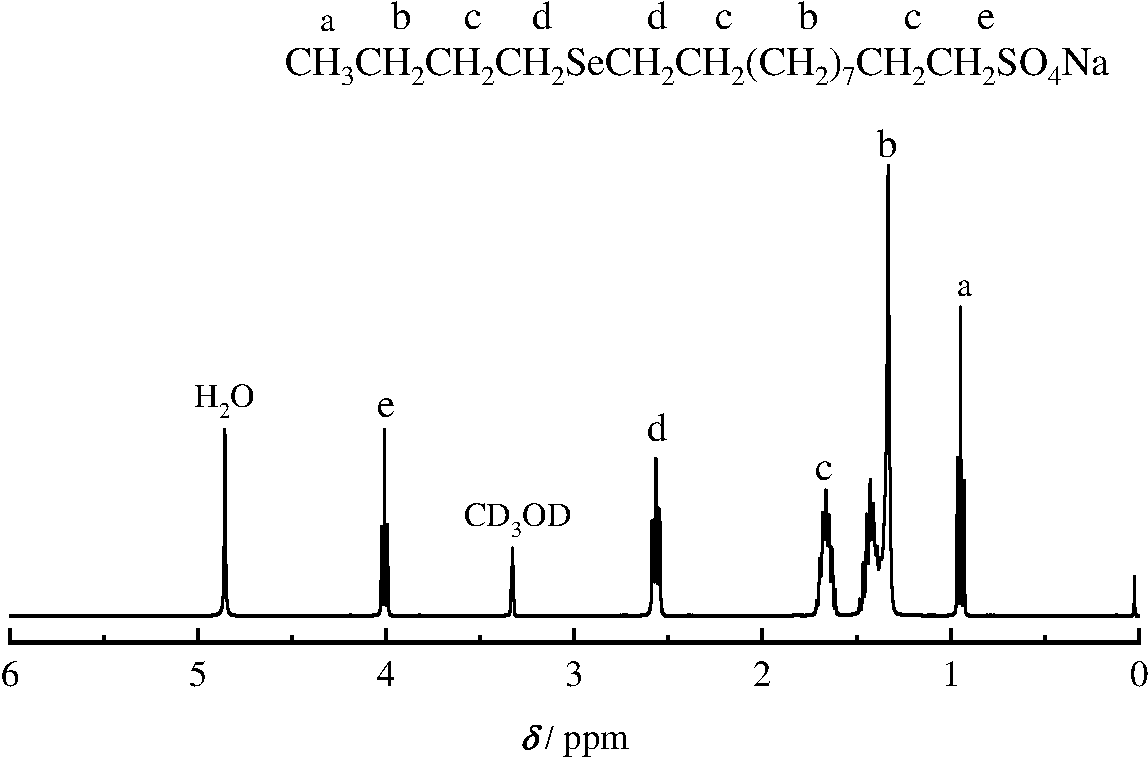
\includegraphics[width=.7\textwidth]{figure/SBSeUS-nmr.pdf}\\
        \caption{SBSeUS的核磁氢谱}\label{fig:SBSeUS-nmr}
    \end{figure}
    
    \ce{^1H} NMR (400 MHz, \ce{CD3OD}, 图\ref{fig:SBSeUS-nmr}) δ 0.95 (t, \textit{J}=7.3 Hz, 3H), 1.27-1.49 (overlap, 16H), 
    1.60-1.73 (m, 6H), 2.52-2.61 (m, 4H), 3.98-4.04 (t, \textit{J}=6.6 Hz, 2H).
    
    对SBSeUS的核磁共振氢谱进行解析,图\ref{fig:SBSeUS-nmr}中,$\delta$ = 3.31的峰为 \ce{CD3OD}溶剂残留峰,
    $\delta$ = 4.87为水峰\cite{波谱解析} ,峰a为 SDSePS 疏水链端甲基的氢信号,以其积分个数为 3 计算,
    实际总氢个数为 31.58,理论氢个数为 31,氢个数基本吻合;峰b为碳链出峰(包括两部分),氢个数为16;
    峰c分别为Se的两端$\beta$位亚甲基氢和极性头基(\ce{-SO4^-})的$\beta$位亚甲基氢出峰\cite{aist},氢个数为6;
    峰d为Se的两端$\alpha$位亚甲基氢出峰\cite{徐辉碧1994,reich1978},氢个数为4;$\delta$ = 4.01处峰e为靠近极性
    头基(\ce{-SO4^-})的亚甲基氢出峰。各峰化学位移与氢个数均可与目标产物对应,由此推断所测样品即为目标产物。
    
    以 \ce{CH3OH}为溶剂,对SDSePS采用负离子模式进行 ESI-MS 测试,测试结果如图\ref{fig:SBSeUS-mass}所示。
    \begin{figure}[htbp]
        \centering
        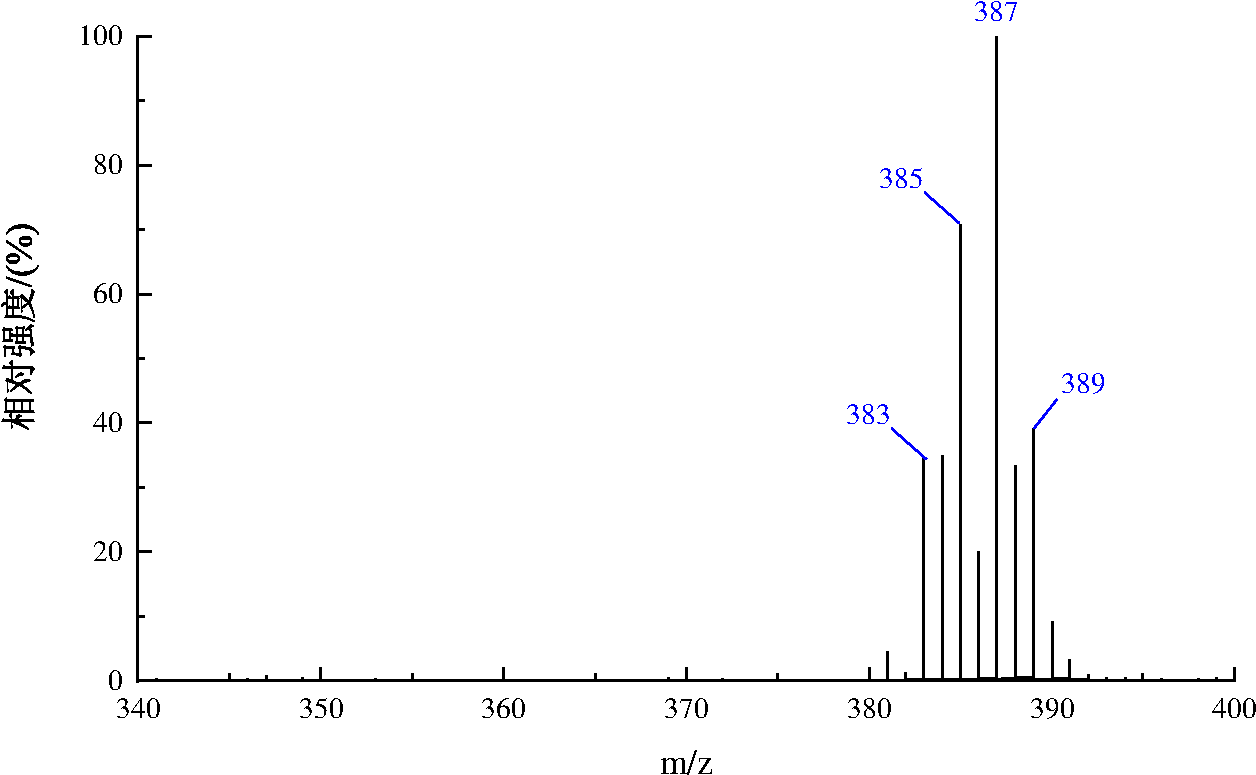
\includegraphics[width=.7\textwidth]{figure/SBSeUS-mass.pdf}\\
        \caption{SBSeUS的质谱}\label{fig:SBSeUS-mass}
    \end{figure}
    
    负离子模式下,相对强度最高的$m/z = 387$的峰应为 \ce{C4H9SeC11H22SO4-}的分子离子峰,与 \ce{C15H31SO4Se}
    的计算结果386.42基本相符,同时硒有多种稳定的同位素,\ce{^74Se} (0.87\%)、\ce{^76Se} (9.02\%)、\ce{^77Se} (7.58\%)、
    \ce{^78Se} (23.52\%)、\ce{^80Se} (49.82\%)、\ce{^82Se} (9.19\%),也与测试结果相符合。

    \section{复配囊泡的构筑}
    \subsection*{(1) SDSePS不同摩尔比}
    将配制好的5 mmol/L的SDSePS水溶液与等浓度的DTAB水溶液以不同摩尔比 (1:9、2:8、3:7、4:6、5:5、6:4、7:3、8:2、9:1)
    复配成总体积5 mL的溶液,混合均匀放置于30 ℃水浴中静置12 h后,外观现象如图\ref{fig:SDSePS-DTAB-ratio}所示,
    可以观察到两端分别是摩尔比较低和较高时溶液更为澄清透明,其中阴阳离子摩尔比为9:1的样品完全澄清,而摩尔比接近
    1的样品呈现不同程度的蓝光(也是囊泡体系的特征之一),摩尔比为7:3和8:2的样品显现蓝光外溶液略显浑浊。
    \begin{figure}[htbp]
        \centering
        \begin{subfigure}[]{\textwidth}
            \centering
            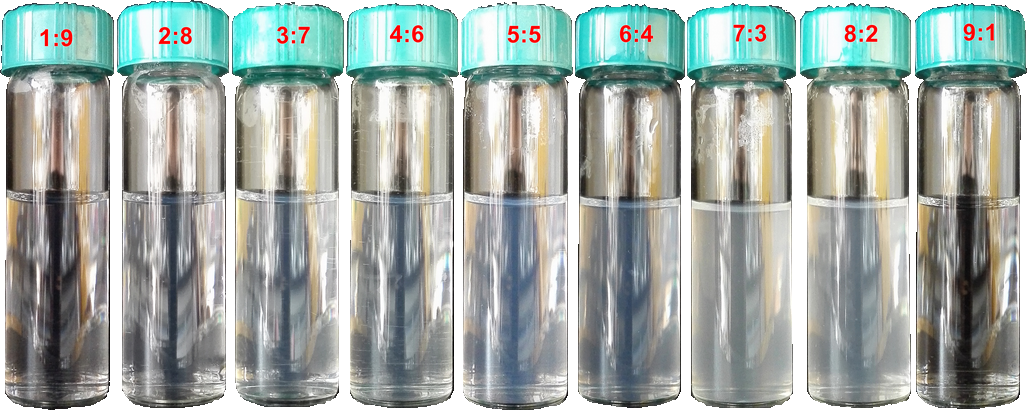
\includegraphics[height=4cm]{figure/SDSePS-DTAB-ratio.png}
            \caption{SDSePS/DTAB不同浓度复配囊泡外观}\label{fig:SDSePS-DTAB-ratio}
        \end{subfigure}%
        
        \begin{subfigure}[]{\textwidth}
            \centering
            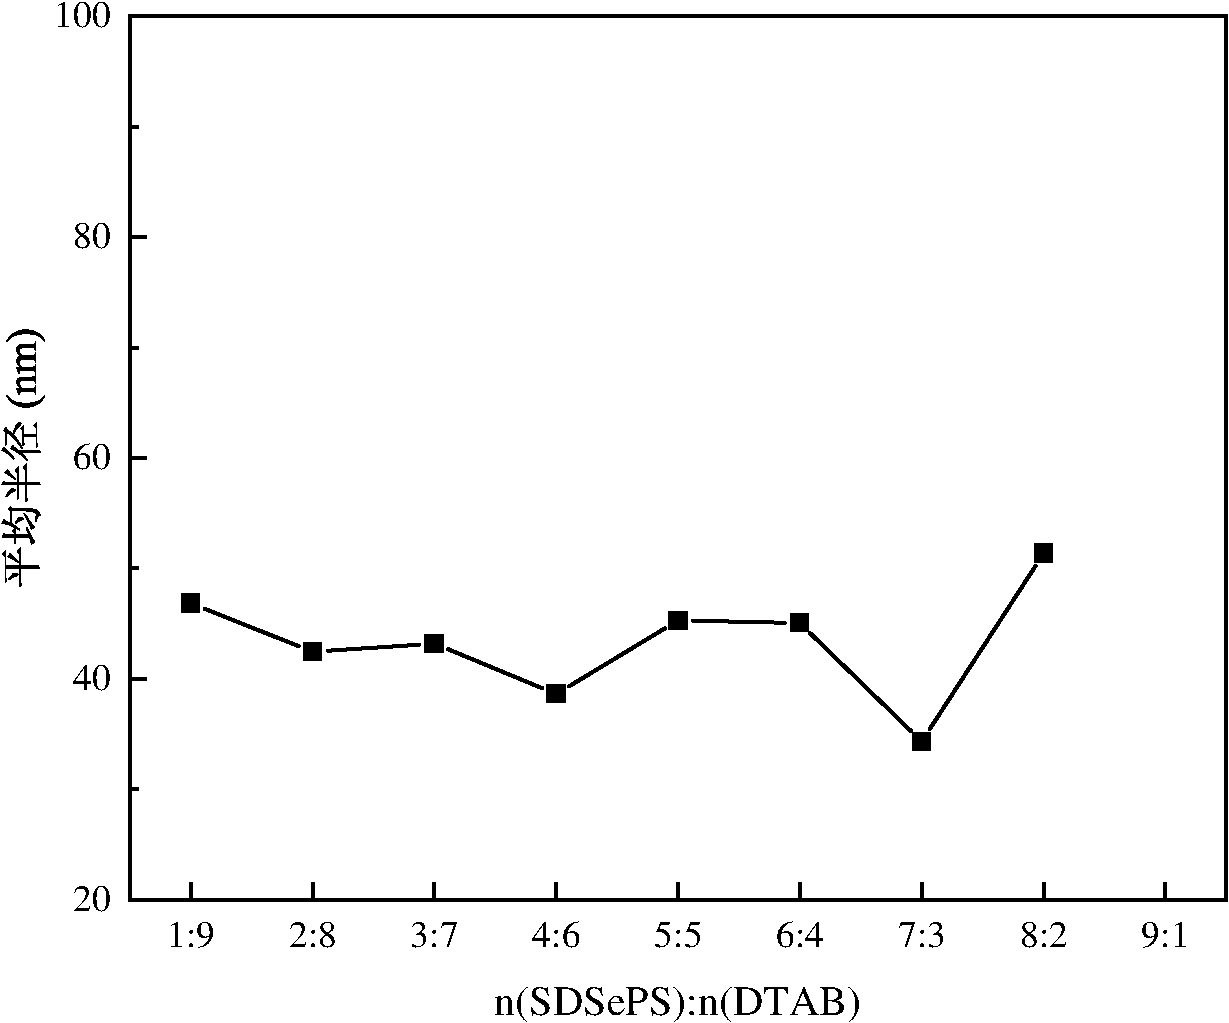
\includegraphics[width=.6\textwidth]{figure/SDSePS-DTAB-ratio-fig.pdf}
            \caption{SDSePS/DTAB不同浓度复配囊泡粒径}\label{fig:SDSePS-DTAB-ratio-fig}
        \end{subfigure}%
        \caption{不同摩尔比SDSePS/DTAB复配体系外观和动态光散射测试结果}
        \label{fig:不同摩尔比SDSePS/DTAB}
    \end{figure}
    所有样品继续恒温静置3天后,摩尔比接近1的5:5和6:4样品产生团絮状沉淀,这应是由于摩尔比接近1时,
    聚集体表面电荷密度更低,仅由离子对解离产生的微弱电荷被溶液中的反离子屏蔽,而聚集体之间的
    静电斥力是保持体系稳定的重要因素,所以此时体系静置后产生团絮状沉淀。
    
    图\ref{fig:SDSePS-DTAB-ratio-fig}为采用动态光散射对上述不同摩尔比的复配体系进行测试的结果,
    结果表明多数样品中均有平均流体力学半径在40-50 nm的聚集体存在,结合复配体系外观呈现蓝色,
    可说明溶液中存在囊泡相。其中摩尔比为9:1的样品的动态光散射结果表明溶液中未检出聚集体的
    存在,其他摩尔比接近1的样品,其平均流体力学半径相对偏低,其中摩尔比7:3的样品最低,为34.32 nm.

    \subsection*{(2) SBSeUS不同摩尔比}
    同SDSePS/DTAB复配体系一样,将配制好的5 mmol/L的SBSeUS水溶液与等浓度的DTAB水溶液
    以不同摩尔比 (1:9、2:8、3:7、4:6、5:5、6:4、7:3、8:2、9:1) 复配成总体积5 mL的溶液,混合均匀,
    放置于30 ℃水浴中静置12 h后,外观现象如图\ref{fig:SBSeUS-DTAB-ratio}所示,同SDSePS/DTAB
    复配体系相似,图中两端位置分别是摩尔比较低和较高时溶液,其更为澄清透明,而摩尔比接近
    1的样品呈现不同程度的蓝光,这说明了可能有囊泡的存在。
    \begin{figure}[htbp]
        \centering
        \begin{subfigure}[]{\textwidth}
            \centering
            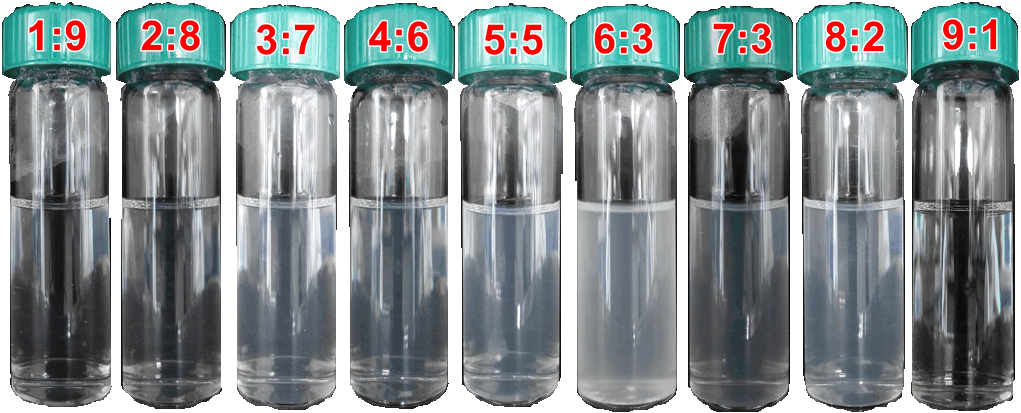
\includegraphics[height=4cm]{figure/SBSeUS-DTAB-ratio.png}\\
            \caption{SBSeUS/DTAB不同浓度复配囊泡外观}\label{fig:SBSeUS-DTAB-ratio}
        \end{subfigure}%

        \begin{subfigure}[]{\textwidth}
            \centering
            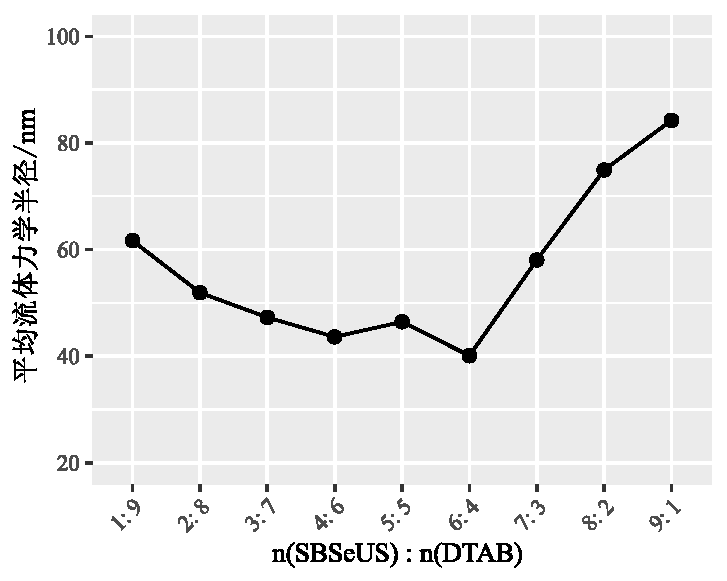
\includegraphics[width=.6\textwidth]{figure/SBSeUS-DTAB-ratio-fig.pdf}\\
            \caption{SBSeUS/DTAB不同浓度复配囊泡粒径}\label{fig:SBSeUS-DTAB-ratio-fig}
        \end{subfigure}%
        \caption{不同摩尔比SBSeUS/DTAB复配体系外观和动态光散射测试结果}
        \label{fig:不同摩尔比SBSeUS/DTAB}
    \end{figure}
    同样,继续长时间放置后,摩尔比接近1的样品会产生团絮状沉淀。
    
    图\ref{fig:SBSeUS-DTAB-ratio-fig}为采用动态光散射对图\ref{fig:SBSeUS-DTAB-ratio}中不同摩尔比的
    复配体系进行测试的结果,结果表明多数样品中均有平均流体力学半径在40-60 nm的聚集体存在,
    结合复配体系外观呈现蓝色的现象,这说明溶液中很有可能存在囊泡相。其中摩尔比为8:2和9:1的
    样品,其平均流体力学半径较大,分别为74.93 nm和84.25 nm.
    
    此外,当阴阳离子表面活性剂摩尔比小于等于4:6时,所构筑的囊泡粒径随摩尔比升高而减小;而当
    摩尔比大于等于6:4时,所构筑的囊泡粒径随摩尔比升高而增大。这可能与阴阳离子表面活性剂形成
    的聚集体的曲率有关,当摩尔比大于等于6:4时,随SBSeUS的增加,复配体系中聚集体曲率增大,从
    而导致聚集体粒径变大\cite{杨成成2017}。
    
    \section{囊泡体系的耐盐性与稳定性}
    分别从耐盐性和随时间的变化两个方面考察阴阳离子表面活性剂复配体系的稳定性。
    
    对于耐盐性,选择以少量多次的方式不断加入 \ce{Na2SO4}直至囊泡相消失,选用 \ce{Na2SO4}是由于本论文中
    设计的含硒阴离子表面活性剂的氧化还原刺激响应性中,采用 \ce{Na2SO3}作为还原剂,会产生
    \ce{Na2SO4}副产物,与此同时,本论文涉及的阴阳离子表面活性剂复配体系为含盐体系(阴阳离子
    表面活性剂带入的反离子),其最多含盐 (NaBr) 不会超过体系浓度的0.5倍 ($0.25 \times 10^{-3}$ mol/L),这相较于加入的 \ce{Na2SO4} 的量非常低。
    
    对于相对时间的稳定性,根据外观现象、动态光散射测试结果及耐盐性选择一个含有囊泡相的最佳摩尔配比,
    采用动态光散射对这一复配体系连续监测其中的聚集体变化。
    
    \subsection*{(1) 耐盐稳定性}
    以少量多次的方式向阴阳离子表面活性剂复配体系SDSePS/DTAB和SBSeUS/DTAB中加入 \ce{Na2SO4},
    直至囊泡相消失,将加入的 \ce{Na2SO4}计算相应的浓度作相图,见图\ref{fig:耐盐相图}。

    \begin{figure}[htbp]
        \centering
        \begin{subfigure}[]{\textwidth}
            \centering
            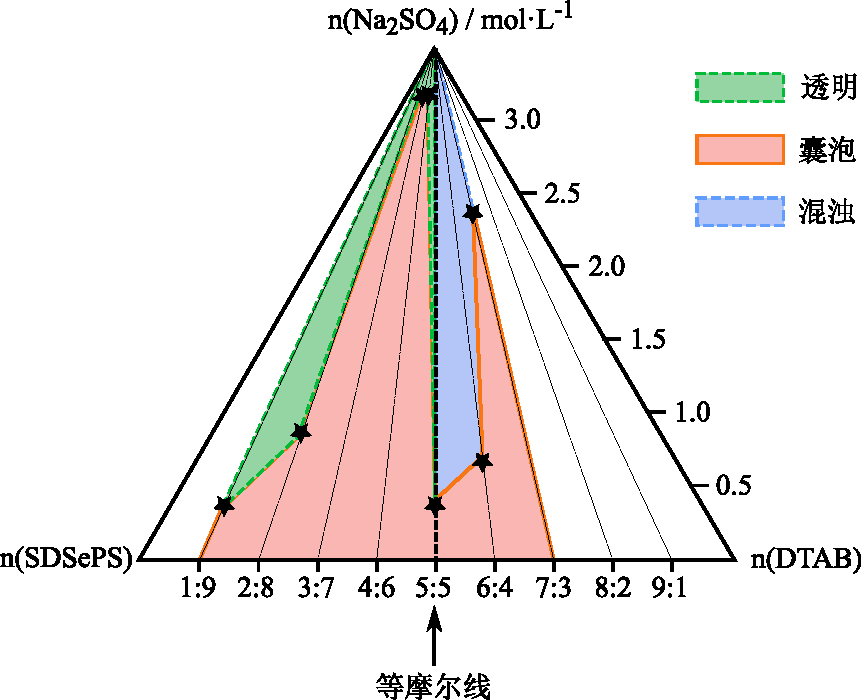
\includegraphics[width=0.52\linewidth]{figure/SDSePS-salt.pdf}
            \caption{SDSePS/DTAB复配体系耐盐相图}\label{fig:SDSePS-salt}
        \end{subfigure}%

        \begin{subfigure}[]{\textwidth}
            \centering
            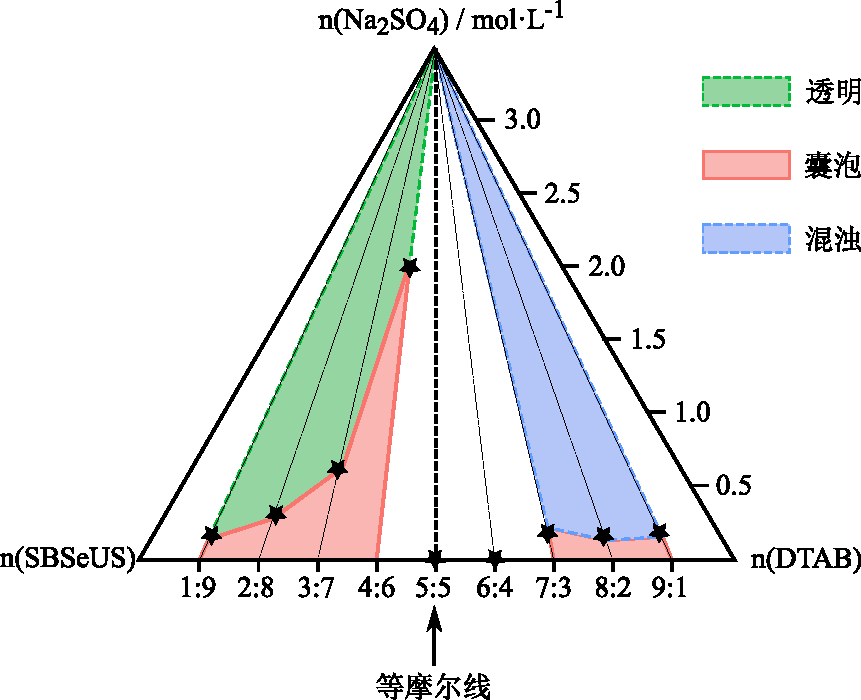
\includegraphics[width=0.52\linewidth]{figure/SBSeUS-salt.pdf}\\
            \caption{SBSeUS/DTAB复配体系耐盐相图}\label{fig:SBSeUS-salt}
        \end{subfigure}%
        \caption{SDSePS/DTAB复配体系及SBSeUS/DTAB复配体系的耐盐相图}
        \label{fig:耐盐相图}
    \end{figure}

    图\ref{fig:SDSePS-salt}为SDSePS/DTAB复配体系的耐盐相图,其中红色部分表示在此
    浓度的 \ce{Na2SO4}存在下,体系尚可保持囊泡相的存在,溶液仍然可见蓝光;绿色和
    蓝色部分则表示加入 \ce{Na2SO4}过量,囊泡相不复存在。而当n(SDSePS):n(DTAB)小于
    1时,当加入 \ce{Na2SO4}过量,即绿色部分,溶液变为澄清透明;当n(SDSePS):n(DTAB)
    大于1时,当加入 \ce{Na2SO4}过量,即蓝色部分,溶液出现浑浊。所有样品中,摩尔比
    为4:6的样品耐盐性最好,可耐受3.10 mol/L \ce{Na2SO4}。
    
    图\ref{fig:SBSeUS-salt}为SBSeUS/DTAB复配体系的耐盐相图,现象基本同SDSePS/DTAB
    复配体系相似,其中红色部分表示在此浓度的 \ce{Na2SO4}存在下,体系尚可保持囊泡相的
    存在;绿色部分表示溶液变为澄清透明;蓝色部分表示溶液出现浑浊。所有样品中,摩尔比
    为4:6的样品耐盐性最好,可耐受1.93 mol/L \ce{Na2SO4},相对于SDSePS/DTAB复配体系,
    SBSeUS/DTAB复配体系的耐盐性偏低。
    
    \subsection*{(2) 粒径随时间变化}
    根据外观现象、动态光散射 (DLS) 和耐盐性测试的结果,选定阴阳离子表面活性剂摩尔比为
    4:6的样品进行SDSePS/DTAB复配体系的后续研究,该配比下体系澄清且蓝光强烈,聚集体
    平均流体力学半径为38.67 nm,存在囊泡相,并且耐盐效果较好。同样标准选择SBSeUS/DTAB
    复配体系的最佳摩尔比为4:6.
    
    对选定配比的阴阳离子表面活性剂体系进行动态光散射测试,对其中的聚集体即囊泡的粒径
    连续测试十天,测试结果见图\ref{fig:vesicle-time-stability}。
    \begin{figure}[htbp]
        \centering
        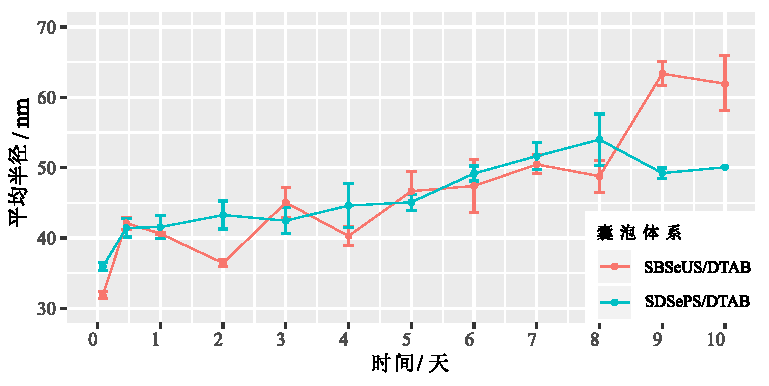
\includegraphics[width=0.7\textwidth]{figure/vesicle-time-stability.pdf}\\
        \caption{复配囊泡稳定性}\label{fig:vesicle-time-stability}
    \end{figure}

    图\ref{fig:vesicle-time-stability}表明SDSePS/DTAB复配体系和SBSeUS/DTAB复配体系中的囊泡
    粒径变化规律基本一致,12 h内囊泡粒径快速上升,之后数天内保持缓慢增长。这与Leng和Cates
    等人提出的自发形成囊泡的动力学过程模型\cite{刘洪国2016}较为符合:前期囊泡形成过程快速,后期
    需要较长时间完成单层囊泡的熟化、分裂和相互融合。图\ref{fig:vesicle-radius}也表明在囊泡的陈化
    过程中,不仅囊泡的平均流体力学半径增加,而且其粒径分布也会变宽。
    \begin{figure}[htbp]
        \centering
        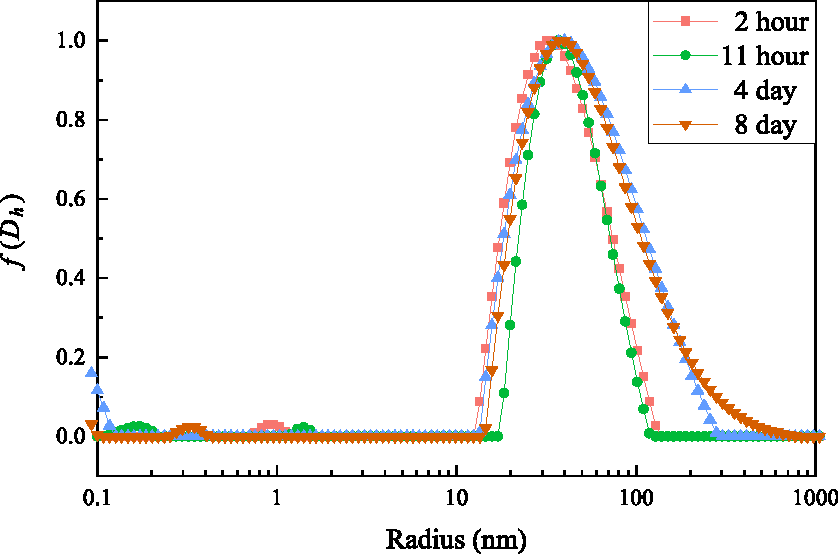
\includegraphics[width=0.675\textwidth]{figure/vesicle-radius.pdf}\\
        \caption{SDSePS/DTAB粒径分布随时间变化}\label{fig:vesicle-radius}
    \end{figure}

    \section{浓度对囊泡体系的影响}
    将先前配制的5 mmol/L、10 mmol/L的SDSePS、SBSeUS和DTAB母液稀释、定容配制一系列
    浓度不等的溶液 (0.5 mmol/L、1 mmol/L、2 mmol/L、2.5 mmol/L、5 mmol/L和10 mmol/L),
    分别按体积比4:6移取同等浓度的SDSePS和DTAB溶液混合得到不同浓度的SDSePS/DTAB复配体系,
    按同样操作制得不同浓度的SBSeUS/DTAB复配体系,于30 ℃恒温静置12 h后所得的外观现象
    如图\ref{fig:不同浓度的复配体系},对其进行动态光散射测试,所得的聚集体粒径结果如图\ref{fig:vesicle-concentration-line}。
    \begin{figure}[htbp]
        \centering
        \begin{subfigure}[]{\textwidth}
            \centering
            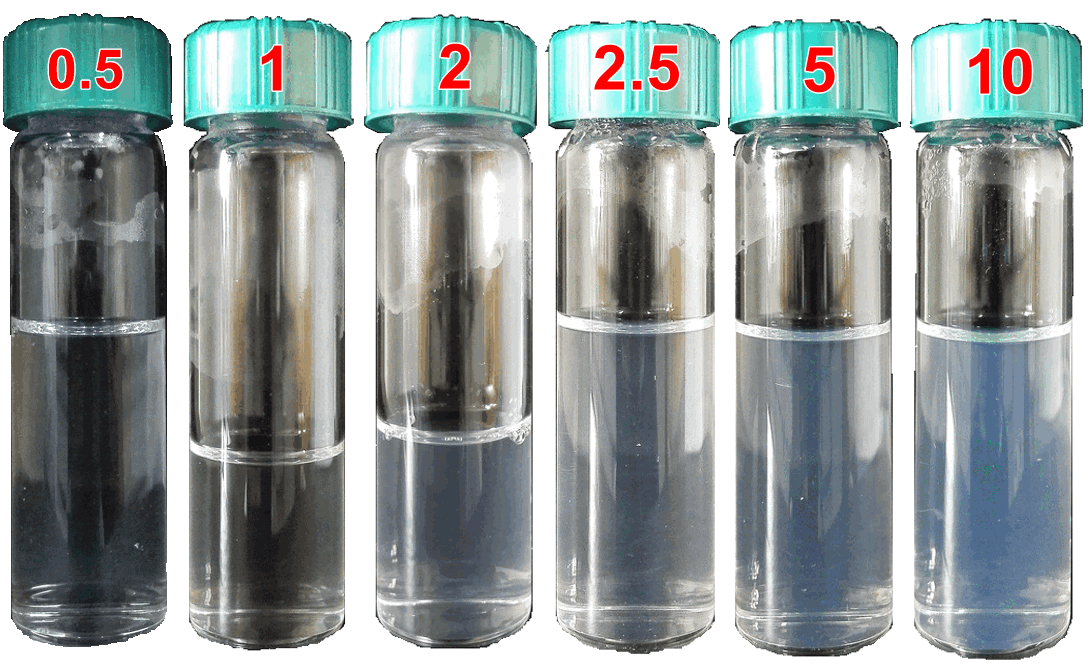
\includegraphics[height=4cm]{figure/SDSePS-concentration.png}\\
            \caption{SDSePS/DTAB不同浓度复配囊泡体系外观}\label{fig:vesicle-SDSePS-concentration}
        \end{subfigure}%
        
        \begin{subfigure}[]{\textwidth}
            \centering
            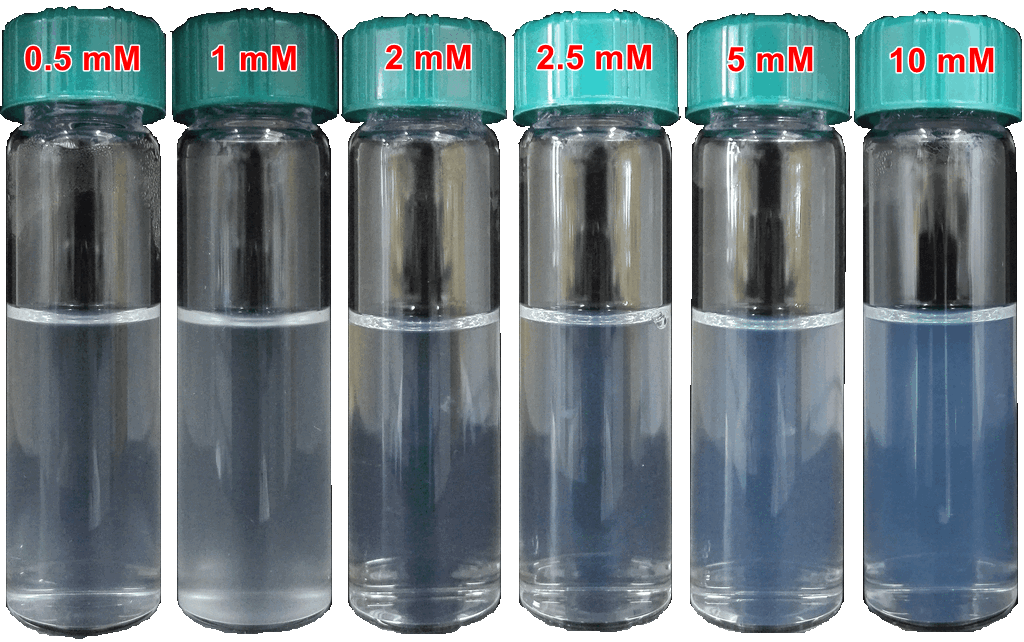
\includegraphics[height=4cm]{figure/SBSeUS-concentration.png}\\
            \caption{不同浓度的SBSeUS/DTAB复配囊泡体系外观}\label{fig:vesicle-SBSeUS-concentration}
        \end{subfigure}%
        \caption{不同浓度的复配体系}
        \label{fig:不同浓度的复配体系}
    \end{figure}
    
    图\ref{fig:vesicle-SDSePS-concentration}和图\ref{fig:vesicle-SBSeUS-concentration}分别
    为不同浓度的SDSePS/DTAB和SBSeUS/DTAB复配体系外观现象,可以看出从浓度为1 mmol/L
    开始复配溶液即开始出现蓝光,而且浓度越高,蓝光愈强。其中SDSePS/DTAB的复配
    体系在较低浓度即1 mmol/L和2 mmol/L时静置后产生少许细密颗粒状沉淀,经0.22 $\mu$m
    水系滤膜过滤后仍可显现蓝光。
    
    \begin{figure}[htbp]
        \centering
        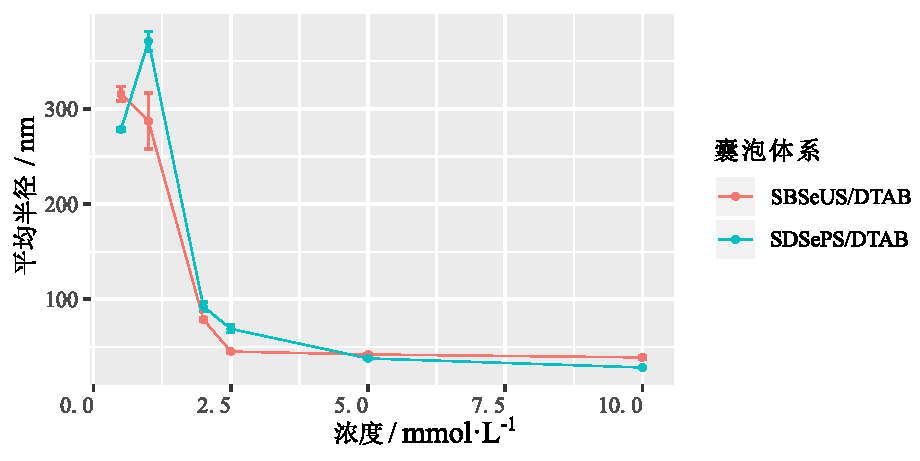
\includegraphics[width=.67\textwidth]{Figure/vesicle-concentration-line.pdf}\\
        \caption{不同浓度复配囊泡粒径变化}\label{fig:vesicle-concentration-line}
    \end{figure}
    
    图\ref{fig:vesicle-concentration-line}显示了SDSePS/DTAB和SBSeUS/DTAB两种复配体系
    中聚集体随着复配溶液浓度的变化情况。其中SDSePS/DTAB复配体系在其浓度小于等于1 mmol/L
    时均存在粒径较大的聚集体存在,这一尺寸的聚集体明显有别于囊泡;当溶液浓度达2 mmol/L时,体系中的
    聚集体尺寸急剧下降到平均流体动力学半径100 nm一下,当浓度达2.5 mmol/L以后,粒径
    变化趋势趋于平缓,基本在40 nm左右,但尺寸继续随浓度升高而降低。SBSeUS/DTAB
    复配体系的粒径及其变化趋势基本同SDSePS/DTAB复配体系一致,这可能是由于碳链中掺杂Se原子
    对表面活性剂分子结构影响不大,因此两种复配体系的性质具有一定相似性。
        
    \section{囊泡体系的氧化还原刺激响应性}
    \subsection{SDSePS/DTAB复配体系的氧化还原响应性}
    向摩尔比为4:6的SDSePS/DTAB复配体系中加入相应于SDSePS 1.2倍量的 \ce{H2O2},30 ℃下
    恒温静置6 h后薄层色谱结果如图\ref{fig:SDSePS-Ox-tlc}所示。
    \begin{figure}[htbp]
        \centering
        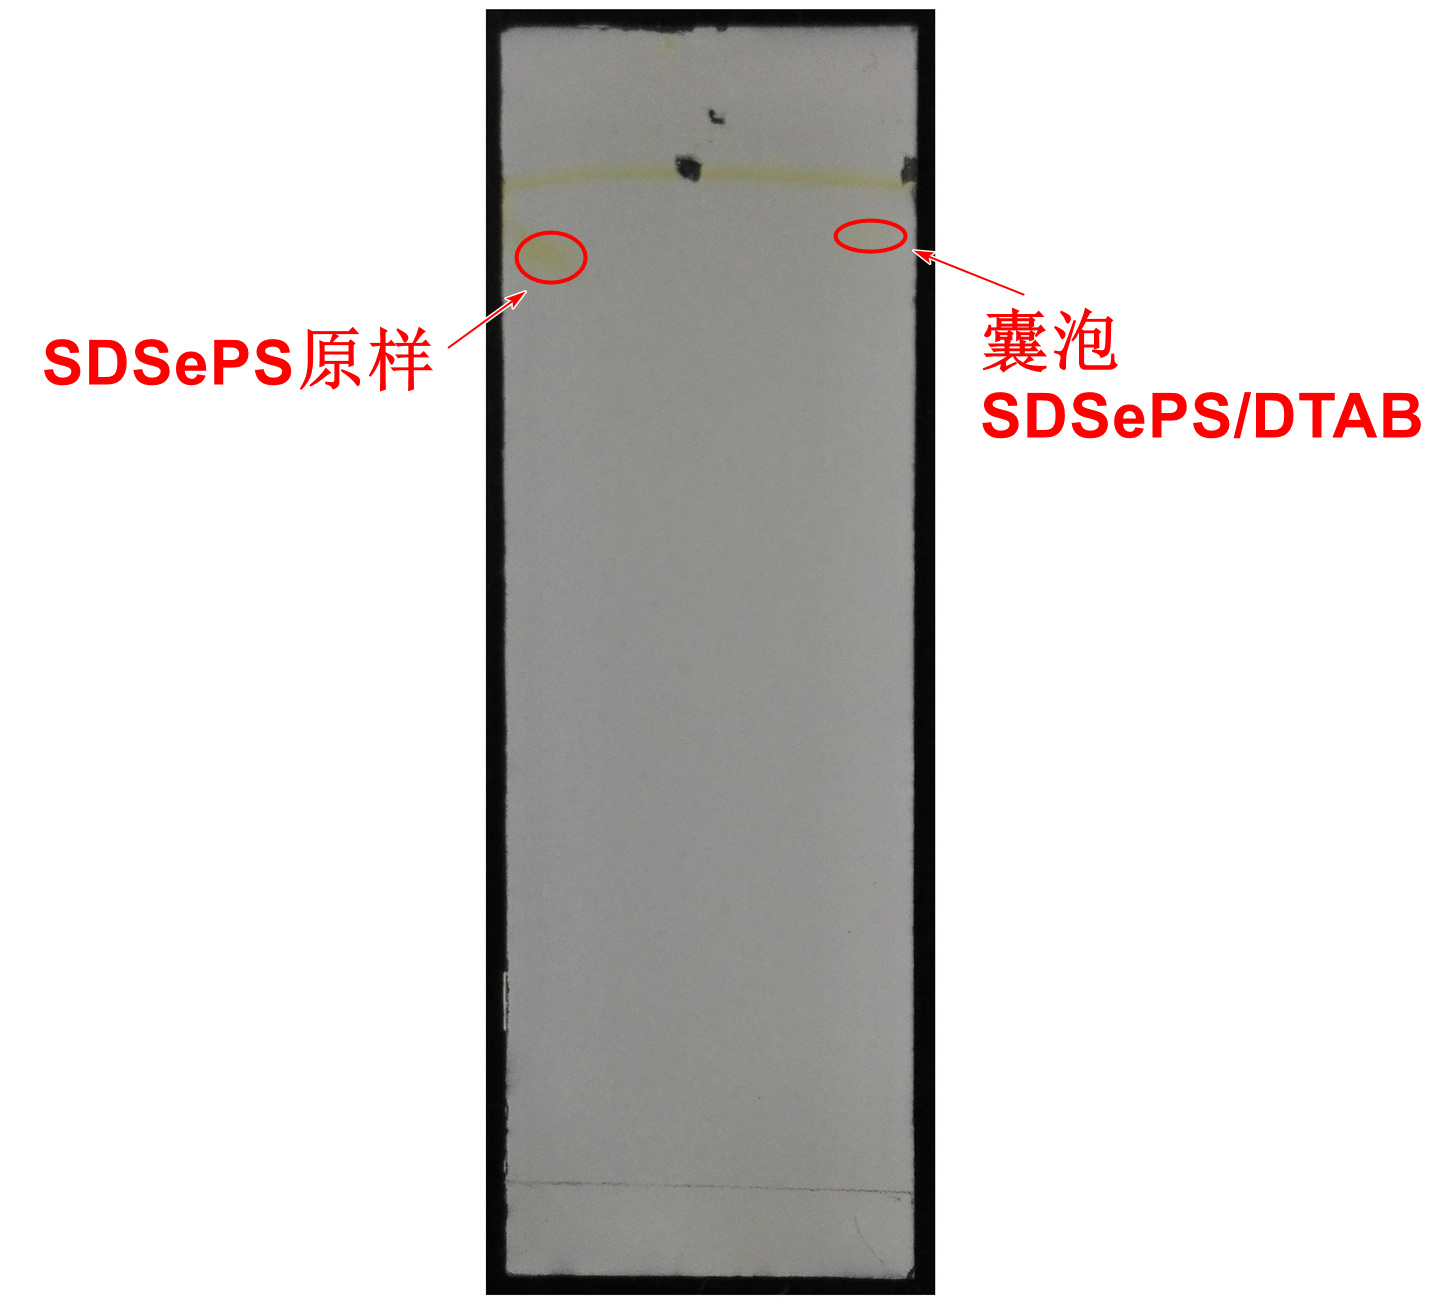
\includegraphics[height=4.5cm]{figure/SDSePS-Ox-tlc.jpg}\\
        \caption{SDSePS氧化完全结果}\label{fig:SDSePS-Ox-tlc}
    \end{figure}
    
    图\ref{fig:SDSePS-Ox-tlc}中左侧点样为提纯的SDSePS样品,中间点样为氧化6 h后的SDSePS/DTAB
    复配体系,右侧点样为SDSePS/DTAB复配体系,中间样品点已不可见SDSePS样品点,说明
    体系中的SDSePS已经氧化完全,图\ref{fig:SDSePS-redox-radius}为氧化循环过程中复配体系中
    聚集体的粒径分布情况,从中也可知氧化完全后,原40 nm左右的囊泡不复存在,仅存在平均流体力学
    半径在3 nm左右的聚集体和少量200 nm的聚集体,前者可能是溶液中的胶束,这可能是由于SDSePS在
    氧化后其亲水头基变大,根据临界堆积参数理论(式\ref{eq:cpp}),此时$p$值减小,因此不再能够构成
    囊泡。
    
    \begin{figure}[htbp]
        \begin{subfigure}[]{.5\textwidth}
            \centering
            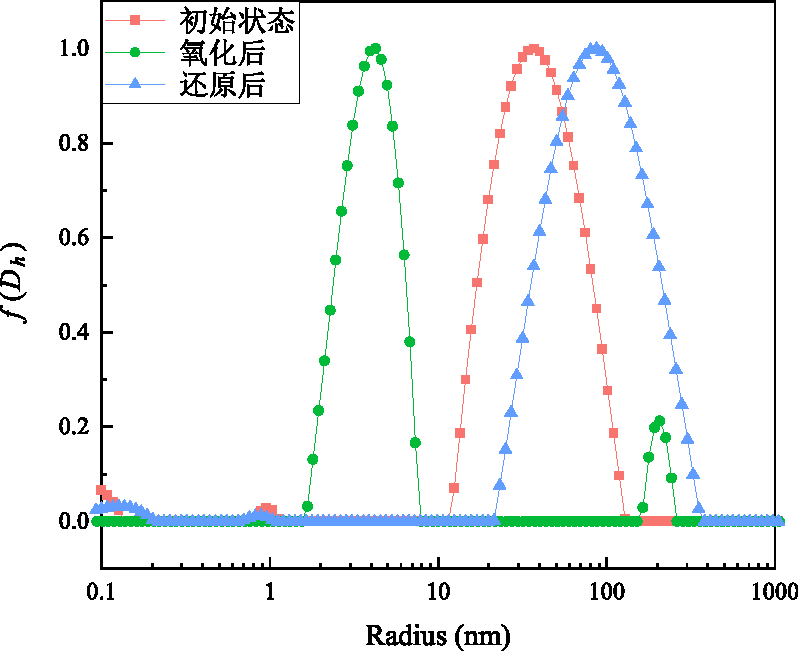
\includegraphics[width=.8\textwidth]{figure/SDSePS-redox-radius.pdf}
            \caption{氧化还原过程中SDSePS/DTAB复配体系\\ 囊泡的粒径变化}\label{fig:SDSePS-redox-radius}
        \end{subfigure}%
        \begin{subfigure}[]{.5\textwidth}
            \centering
            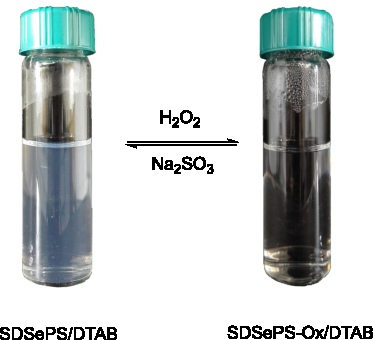
\includegraphics[height=4.5cm]{figure/scheme-SDSePS-redox.pdf}
            \caption{SDSePS/DTAB复配体系在氧化还原后的外观现象}\label{fig:scheme-SDSePS-redox}
        \end{subfigure}%
        \caption{氧化还原刺激响应性}
        \label{fig:氧化还原刺激响应性}
    \end{figure}
    
    向经 \ce{H2O2}氧化过的复配体系中加入1.2倍阴离子表面活性剂的量的 \ce{Na2SO3}进行还原,还原后
    溶液恢复蓝色外观,其中的聚集体粒径分布变化见图\ref{fig:SDSePS-redox-radius},从中可知聚集体基本
    恢复到原有尺寸范围,但相较于原来略大。
%    \begin{figure}[htbp]
%        \centering
%        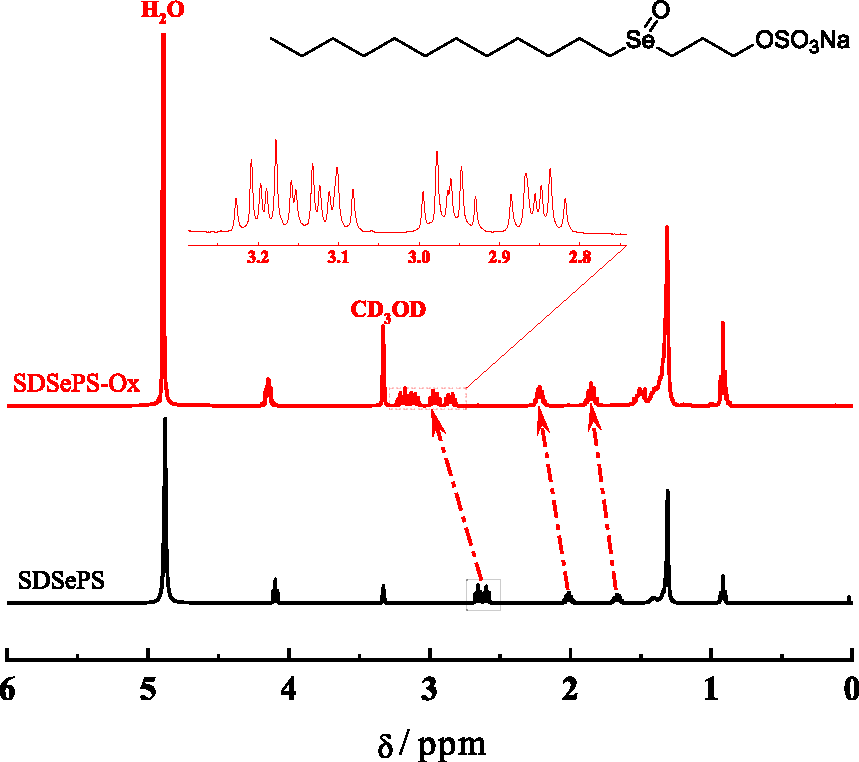
\includegraphics[width=.4\textwidth]{figure/SDSePS-nmr-diff.pdf}\\
%        \caption{12+3对比核磁}\label{fig:SDSePs-nmr-diff}
%    \end{figure}
    
    针对还原后的体系连续监测其中的聚集体变化10天,其变化图\ref{fig:vesicle-Re-stability},可知还原的
    过程可能十分迅速,10 min后监测其中的粒径分布,仅有约40 nm左右的范围内存在聚集体分布。在随后
    的数日内聚集体粒径缓慢增长,基本在1天后聚集体即保持相对稳定。
    
    \begin{figure}[htbp]
        \centering
        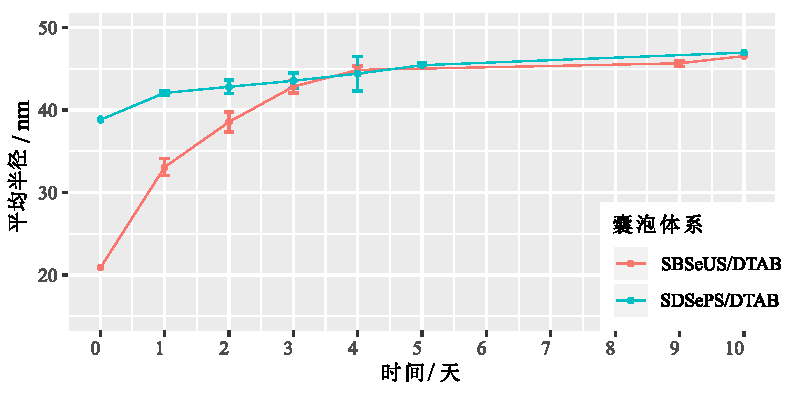
\includegraphics[width=.6\textwidth]{figure/vesicle-Re-stability.pdf}\\
        \caption{一次还原稳定性}\label{fig:vesicle-Re-stability}
    \end{figure}
    
    对SDSePS/DTAB复配体系连续进行10次的氧化还原过程,采用动态光散射测试其中的聚集体结果
    见图\ref{fig:SDSePS-redox-circle}。
    \begin{figure}[htbp]
        \centering
        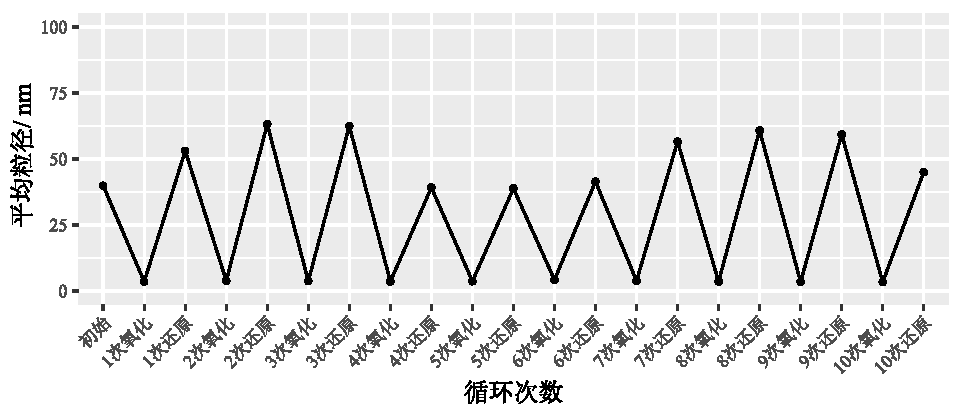
\includegraphics[width=.86\textwidth]{figure/SDSePS-redox-circle.pdf}\\
        \caption{SDSePS/DTAB复配囊泡体系氧化还原循环过程中的粒径变化}\label{fig:SDSePS-redox-circle}
    \end{figure}
    从中可知构筑的SDSePS/DTAB囊泡具有很好的氧化还原刺激响应性,能够进行多次的氧化还原循环,
    在囊泡和胶束的聚集体结构之间切换。仅从耐盐性的角度看(图\ref{fig:SDSePS-salt}),这一复配体系
    可以进行近1300次氧化还原过程。
    
    \subsection{SBSeUS/DTAB复配体系的氧化还原响应性}
    向摩尔比为4:6的SBSeUS/DTAB中加入1.2倍 \ce{H2O2},恒温30 ℃静置,发现需经 72 h后体系方呈澄清透明,
    相同条件下于40 ℃恒温静置进行氧化,需要42 h体系方呈澄清透明。相比于SDSePS/DTAB复配体系,
    发现氧化过程明显更加困难,这可能是由于SBSeUS/DTAB复配体系中形成了囊泡这一聚集体结构(见示意图\ref{fig:scheme-vesicle}),
    相较于SDSePS中Se原子更加靠近亲水头基(图\ref{fig:scheme-synthesis}),易于被 \ce{H2O2}氧化,SBSePS
    中Se原子处于疏水尾链中,形成囊泡后Se原子位于双分子层内部,不易于氧化。同时相同条件下,同浓度的
    表面活性剂SBSeUS的水溶液在40 ℃下5 h内即可完成氧化,这也印证了以上说法。以上实验中氧化完全与否
    均采用薄层色谱监测。
    \begin{figure}[htbp]
        \centering
        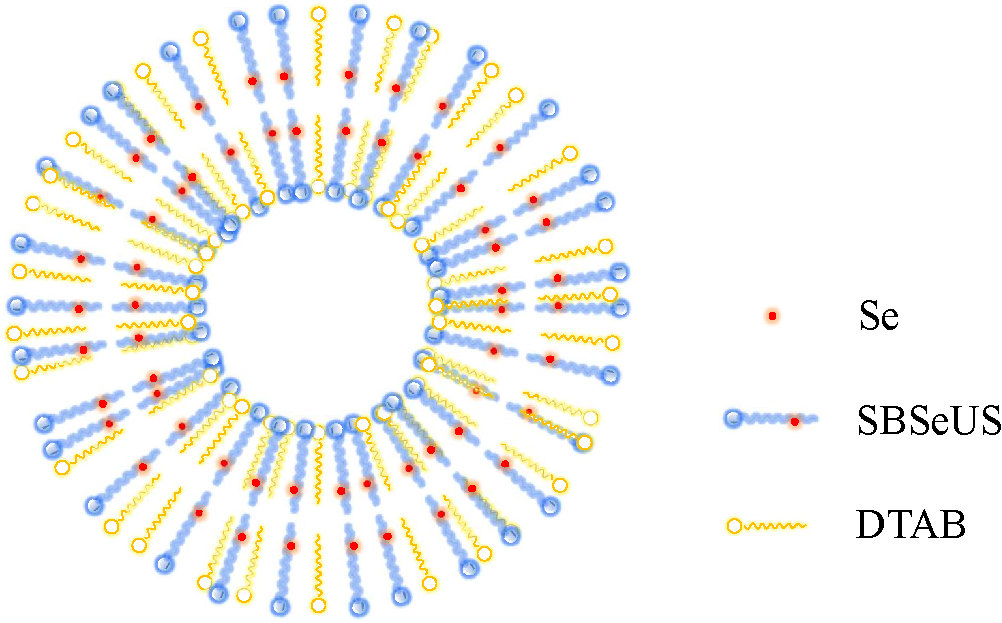
\includegraphics[width=0.4\linewidth]{figure/vesicle-scheme.pdf}\\
        \caption{SBSeUS/DTAB囊泡示意图}\label{fig:scheme-vesicle}
    \end{figure}
    
    继续增加 \ce{H2O2} 浓度,发现2.0倍 \ce{H2O2} 可在40 ℃下24 h可将SBSeUS/DTAB复配体系囊泡
    瓦解,薄层色谱结果显示表面活性剂SBSeUS已被氧化完全,见图\ref{fig:SBSeUS-Ox-tlc},此时复配
    体系澄清透明,见图\ref{fig:scheme-SBSeUS-redox},蓝光消失,说明体系中的囊泡可能已经瓦解。
    采用动态光散射测试氧化后的复配体系,测试结果见图\ref{fig:SBSeUS-redox-radius},从中可以看出
    氧化后体系中主要有两个范围内有聚集体存在,其中3 nm左右的应为胶束相,另外在200 nm以上
    也检测出聚集体存在,这一现象与SDSePS/DTAB复配体系氧化后类似,但200 nm以上区域存在的
    聚集体更加多。
    \begin{figure}[htbp]
        \centering
        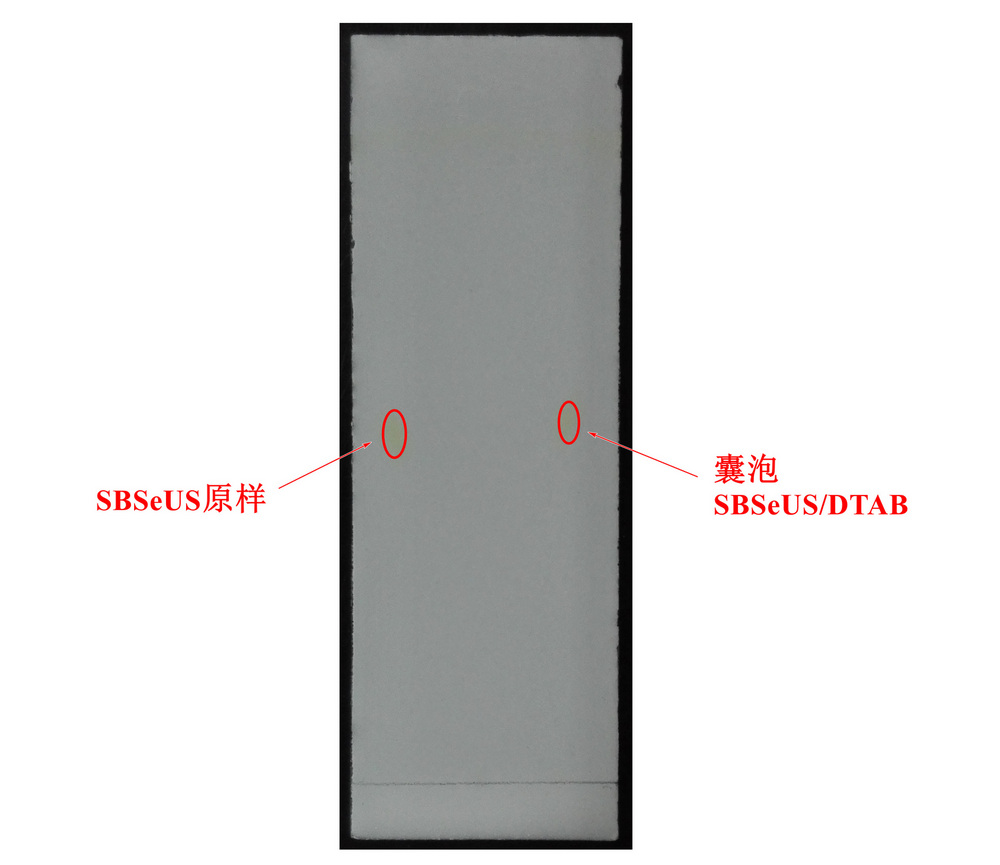
\includegraphics[height=5.5cm]{figure/SBSeUS-Ox-tlc}\\
        \caption{SBSeUS 氧化完全结果}\label{fig:SBSeUS-Ox-tlc}
    \end{figure}
    
    将上述氧化后的体系采用2.0倍 \ce{Na2SO3} 进行还原,氧化还原过程中的外观变化及体系内聚集体
    分布变化见图\ref{fig:SBSeUS/DTAB氧化还原刺激响应性},对还原后的复配体系中的聚集体连续使用
    动态光散射监测10天,结果见图\ref{fig:vesicle-Re-stability}。还原后的体系10 min后即仅监测到20 nm左右范围存在较窄的
    粒径分布,还原后的体系需3天后方能进入较稳定的状态,稳定后的SBSeUS/DTAB体系中的囊泡粒径
    与还原后的SDSePS/DTAB中囊泡粒径较为接近,均在47 nm左右。
    \begin{figure}[htbp]
        \begin{subfigure}[]{.5\textwidth}
            \centering
            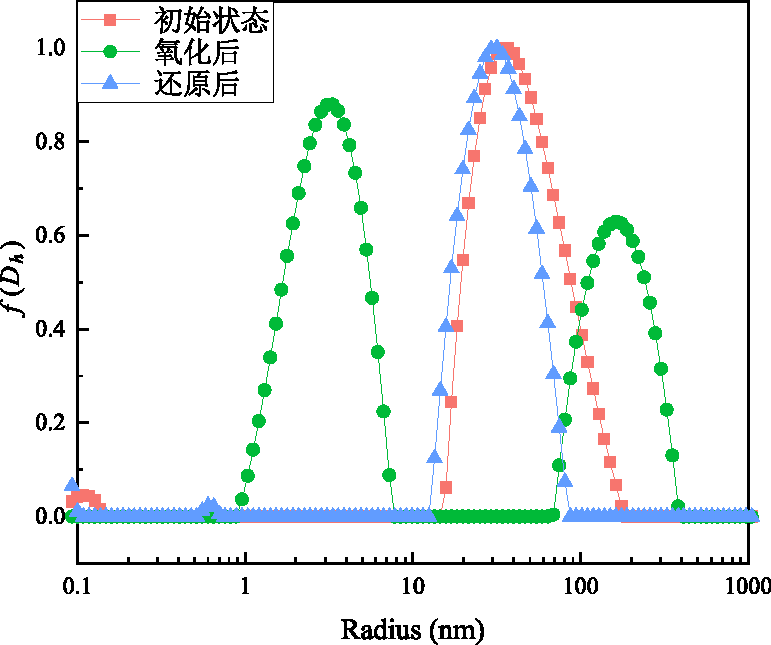
\includegraphics[width=.8\textwidth]{figure/SBSeUS-redox-radius.pdf}
            \caption{氧化还原过程中SBSeUS/DTAB复配体系\\囊泡的粒径变化}\label{fig:SBSeUS-redox-radius}
        \end{subfigure}%
        \begin{subfigure}[]{.5\textwidth}
            \centering
            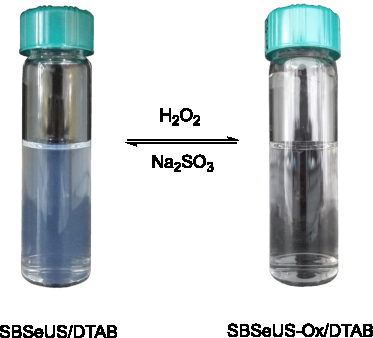
\includegraphics[height=4.5cm]{figure/scheme-SBSeUS-redox.pdf}
            \caption{SBSeUS/DTAB复配体系在氧化还原后的外观现象}\label{fig:scheme-SBSeUS-redox}
        \end{subfigure}%
        \caption{氧化还原刺激响应性}
        \label{fig:SBSeUS/DTAB氧化还原刺激响应性}
    \end{figure}
    
    对SBSeUS/DTAB进行了3次的氧化还原循环,可见这一体系也具有氧化还原刺激响应性,但从氧化过程
    看,其氧化还原刺激响应性能次于SDSePS/DTAB复配体系。
    \begin{figure}[htbp]
        \centering
        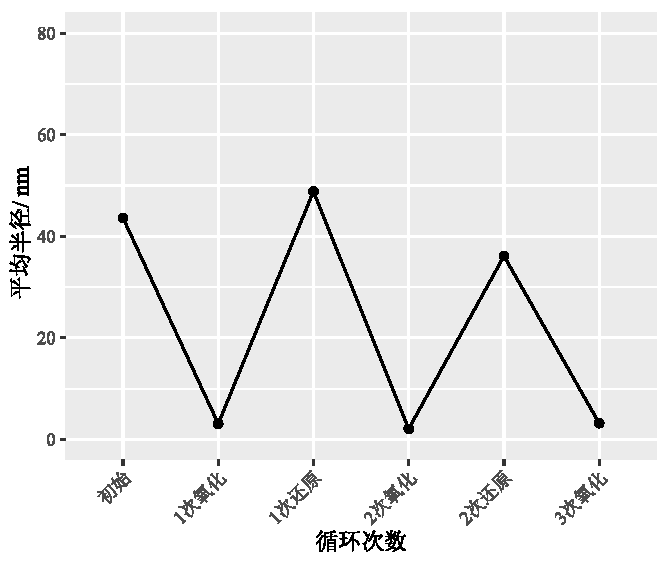
\includegraphics[width=.4\textwidth]{figure/SBSeUS-redox-circle}\\
        \caption{SBSeUS/DTAB复配囊泡体系氧化还原循环过程中的粒径变化}\label{fig:SBSeUS-redox-circle}
    \end{figure}
    
    %%%%%%%%%%%%%%%%%%%%%%%%%%%%%%%%%%%%%%%%%
    % 学位论文的正文应以《结论》作为最后一章
    \chapter{结论与展望}\label{chapter:concludes}
    \section{结论}
    本论文制备了两种含硒阴离子表面活性剂3-十二烷基硒-1-丙基硫酸钠 (SDSePS) 和11-丁基
    硒-1-十一烷基硫酸钠 (SBSeUS),利用含硒阴离子表面活性剂与阳离子表面活性剂 (DTAB)
    进行复配得到两种自发形成的囊泡体系,考察了自发囊泡形成的复配摩尔比及浓度,研究了复配体系
    的耐盐性与稳定性,着重考察了自发形成囊泡的氧化还原刺激响应性能,所得结论如下:
    \begin{enumerate}
        \item 在摩尔比1:9至9:1的范围内,SDSePS、SBSeUS均能与DTAB自发形成囊泡,但是
        在接近摩尔比为1时,形成的复配体系不稳定,放置数日即产生沉淀;
        \item 复配体系SDSePS/DTAB和SBSeUS/DTAB均当浓度大于等于2.5 mmol/L时可形成囊泡,
        并且在2.5-10 mmol/L的范围内,所形成的囊泡粒径缓慢降低;
        \item 复配体系SDSePS/DTAB和SBSeUS/DTAB耐盐性最好的阴阳离子表面活性剂复配摩尔比
        均为4:6,复配形成的囊泡具有相当的稳定性;
        \item 复配体系SDSePS/DTAB较SBSeUS/DTAB易于氧化,在氧化剂和还原剂的调控下可实现
        体系内囊泡相和胶束相的可逆转变。
    \end{enumerate}
        
    \section{展望}
    本论文利用含硒阴离子表面活性剂与阳离子表面活性剂复配形成了自发囊泡,并且复配体系
    SDSePS/DTAB具有很好的氧化还原刺激响应性,但还存在一些问题需要研究和解决:
    \begin{enumerate}
        \item 在较低浓度如1 mmol/L附近复配时,两种复配体系均会产生细微沉淀,而当在更低或高浓度
        时,体系均保持澄清透明,这一点需要加以验证;
        \item 复配体系SBSeUS/DTAB虽然其氧化过程难于SDSePS/DTAB,但适当条件下其仍可以实现
        较好的氧化,本论文使用较高浓度的 \ce{H2O2} 进行氧化,对于其氧化条件、氧化产物和囊泡瓦解
        的机制也值得探索。
    \end{enumerate}
    
    \begin{backmatter}
    \fancyhead[C]{\songti\zihao{-5}参考文献}
    % 推荐使用BibTeX,若不使用BibTeX时注释掉下面一句。
    %\nocite{*}
    \bibliography{bachelor}
    \end{backmatter}

%%%%%%%%%%%%%%%%%%%%%%%%%%%%%%%%%%%%%%%%%%%%%%%%%%%%%
% 致谢,应放在《结论》之后
    \begin{acknowledgement}
        \fancyhead[C]{\songti\zihao{-5}致谢}
        首先感谢我的指导教师刘雪锋老师,此次毕业设计从开题到实验方案的拟定、从实验过程到
        毕业论文的撰写,无不是在刘老师的悉心指导下完成的,感谢刘老师传授的宝贵经验和建议;
        
        接下来,感谢李颖学姐和刘德琼学姐,她们对我的实验开展提供了细致、及时的指导与帮助,感谢
        刘德琼学姐阅读了我的论文草稿,提出了宝贵的修改建议;同时感谢化工楼B503的研究生
        师兄师姐们,是他们提供了友好的实验氛围与日常帮助;
        
        再者,还要感谢与我一同开展毕设设计的王樊、王淑钰、许馨瑶同学,感谢他们在毕业设计期间
        提供的帮助与扶持;
        
        最后,感谢我的父母对我二十多年来的养育之恩,感谢他们对我学业上的支持和生活上的包容,
        谢谢您们!
    \end{acknowledgement}
    
%\begin{backmatter}
%\fancyhead[C]{\songti\zihao{-5}附录}
%\chapter{附录 A:彩色插图}
%\begin{figure}[htbp]
%    \centering
%    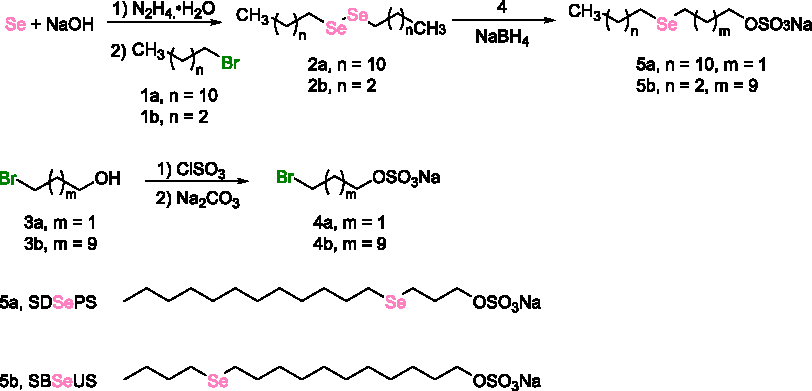
\includegraphics[scale=1]{figure/scheme-synthesis.pdf}\\
%    \caption{含硒表面活性剂的合成路线}
%\end{figure}
%\end{backmatter}
%%%%%%%%%%%%%%%%%%%%%%%%%%%%%%%%%%%%%%%%%%%%%%%%%%%
\end{document}